% Do not forget to include Introduction
%---------------------------------------------------------------
% \chapter{Introduction}
% uncomment the following line to create an unnumbered chapter
\chapter*{Úvod}
\addcontentsline{toc}{chapter}{Úvod}
\markboth{Úvod}{Úvod}
%---------------------------------------------------------------
\setcounter{page}{1}

% The following environment can be used as a mini-introduction for a chapter. Use that any way it pleases you (or comment it out). It can contain, for instance, a summary of the chapter. Or, there can be a quotation.
%\begin{chapterabstract}
%	\lipsum[1]
%\end{chapterabstract}

%Software je součástí důležitých systémů jako například ovládací a monitorovací prvky v letadlech, autech či zdravotnických zařízeních. Software dnes provádí bankovní transakce,  zabezpečení a šifrování tajných zpráv. 

Vývoj softwaru počítače doprovází také neúmyslně vznikající chyby. Nejznámější softwarové chyby způsobily například havárii nosné rakety Ariane 5 při zkušebním letu v roce 1996, ztrátu satelitu Mars Climate Orbiter nebo smrt šesti pacientů zdravotnického přístroje Therac-25. Všechny tyto a další podobné případy spojuje chybně naprogramovaný software počítače.

Aktivita, která má za účel minimalizovat výskyt těchto chyb se nazývá softwarové testování. Principem tohoto testování je vyzkoušet naprogramovaný algoritmus v kontrolovaném prostředí na velkém množství kombinací vstupních parametrů a zajistit, že kód generuje správné výsledky. Slavný citát Edsgera Wybe Dijkstry zní: \uv{Testováním programu lze prokázat existenci chyby, nikoli její nepřítomnost}. V praxi se často používá metoda testování softwaru, která pokrývá pouze podmnožinu všech možných kombinací vstupních parametrů. Tento styl testování softwaru zajišťuje primárně kontrolu funkčnosti při následné modifikaci zdrojového kódu. \uv{Test driven development} označuje metodu vývoje softwaru, při které jsou  testovací scénáře vytvářeny dříve, než samotný kód. Tato metoda zajišťuje pokrytí testovacími scénáři velké části výsledného software, ale stále nezajišťuje korektnost daného algoritmu. \cite{TDD2002}

Statická analýza kódu kontroluje zdrojový kód algoritmu a z kódu odvozuje některé vlastnosti bez nutnosti spuštění daného kódu. Formální analýza je rozšířením statické analýzy o možnost definovat vlastnosti vstupních parametrů, výstupních hodnot a možnost provádět induktivní důkazy za pomocí cyklů. Tato metodika testování korektnosti algoritmů bude v této práci aplikována na datovou strukturu binární minimové haldy.

Binární minimová halda je jedna ze základních datových struktur. Halda se používá například k implementaci prioritní fronty. Jednotlivé prvky jsou tedy řazeny dle jejich priority. Tato struktura lze následně použít v Dijkstrově algoritmu pro hledání nejkratší cesty v grafu.

Tato práce zkoumá jednotlivé operace nad binární minimovou haldou a vysvětluje postup tvorby formálních důkazů v jazyce ACSL. Hlavním cílem této práce je vytvoření kompletní softwarové knihovny v programovacím jazyce C implementující operace nad binární minimovou haldou, opatřit jednotlivé operace v této knihovně ACSL anotacemi a provést formální důkaz korektnosti daných algoritmů v prostředí Frama-C.

%---------------------------------------------------------------
\chapter{Binární halda}
%---------------------------------------------------------------

Tato kapitola shrnuje základní pojmy teorie grafů, které tvoří podklady pro následující kapitoly. V průběhu textu je pojem vrchol haldy a prvek haldy považován za ekvivalentní.

\begin{definition}[Souvislý graf]
Graf $G = (V, E)$ je souvislý, jestliže v něm pro každé jeho dva vrcholy u, v existuje u-v-cesta.
\end{definition}

\begin{definition}[Strom]
Graf $G = (V, E)$ nazveme stromem, pokud je souvislý a neobsahuje žádnou kružnici (čili je acyklický).
\end{definition}

\begin{definition}[Binární strom]
Strom nazveme \textit{binární}, pokud je \textit{zakořeněný} a každý vrchol má nejvýše dva
syny, u nichž rozlišujeme, který je levý a který pravý. Vrcholy rozdělíme podle vzdálenosti
od kořene do hladin: v nulté hladině leží kořen, v první jeho synové atd.
\end{definition}

\begin{definition}[Binární minimová halda]
\label{definition:binary-min-heap}
\textit{Binární minimová halda} je datová struktura tvaru binárního stromu, v jehož
každém vrcholu je uložen jeden prvek. Přitom platí:
\begin{enumerate}
	\item[] Tvar haldy: Všechny hladiny kromě poslední jsou plně obsazené. Poslední hladina je
zaplněna zleva.
	\item[] Haldové uspořádání: Je-li $u$ vrchol a $v$ jeho syn, platí: $\Value(u) \leq \Value(v)$.
\end{enumerate}

\end{definition}

\begin{figure}[H]
	\centering
	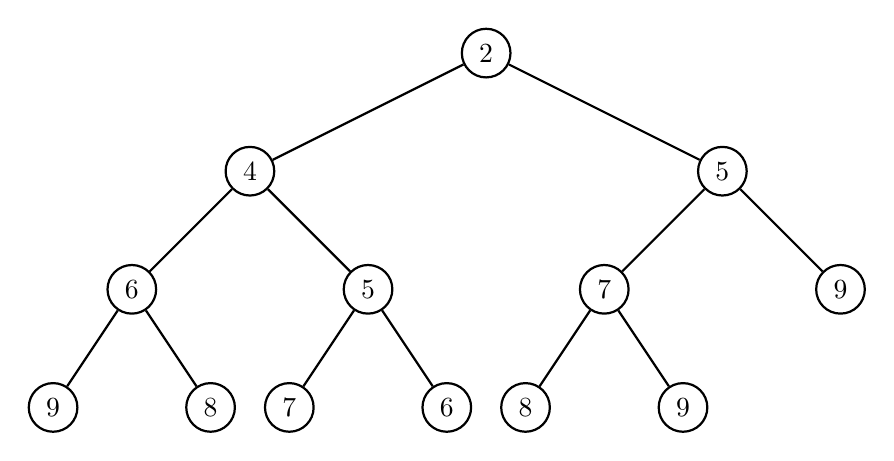
\begin{tikzpicture}[level/.style={sibling distance=60mm/#1}]
		\node [circle,thick,draw] (0) {2}
		child[thick] { node [circle,draw] (1) {4}
			child { node [circle,draw] (3) {6}
				child { node [circle,draw] (7) {9} }
				child { node [circle,draw] (8) {8} }
			}
			child { node [circle,draw] (4) {5}
				child { node [circle,draw] (9) {7} }
				child { node [circle,draw] (10) {6} }
			}
		}
		child[thick] { node [circle,draw] (2) {5}
			child { node [circle,draw] (5) {7}
				child { node [circle,draw] (11) {8} }
				child { node [circle,draw] (12) {9} }
			}
			child { node [circle,draw] (6) {9} }
		};
	\end{tikzpicture}
	\caption{Ukázka binární minimové haldy}
	\label{img:heap-example}
\end{figure}

\pagebreak

Obrázek \ref{img:heap-example} zobrazuje ukázku binární minimové haldy. Haldu lze uložit do lineárního pole, kde kořen haldy je uložen na indexu $0$. Haldu z obrázku \ref{img:heap-example} implementovaná pomocí pole je vidět na obrázku \ref{img:heap-example-array}. Průchod haldou lze realizovat následujícími aritmetickými operacemi:

\begin{enumerate}
	\item[] $\Parent(i) = \lfloor (i - 1) / 2 \rfloor$
	\item[] $\LeftChild(i) = 2i + 1$
	\item[] $\RightChild(i) = 2i + 2$
\end{enumerate}

\begin{figure}[H]
	\centering
	\begin{tikzpicture}
	\matrix (m) [matrix of nodes,
	             nodes={draw, minimum size=8mm,anchor=center},
	             nodes in empty cells, minimum height = 1cm,
	             row 1/.style={nodes={draw=none}},]
	{
	  0 & 1 & 2 & 3 & 4 & 5 & 6 & 7 & 8 & 9 & 10 & 11 & 12  \\
	  2 & 4 & 5 & 6 & 5 & 7 & 9 & 9 & 8 & 7 & 6 & 8 & 9 \\
	};
	\end{tikzpicture}
	\caption{Ukázka uložení binární minimové haldy v poli}
	\label{img:heap-example-array}
\end{figure}

%---------------------------------------------------------------
\chapter{ACSL a verifikační prostředí}
%---------------------------------------------------------------

\section{ACSL}

ACSL je akronym pro \uv{ANSI/ISO C Specification Language}. Algoritmy v jazyce C lze anotovat pomocí jazyka ACSL a následně provádět statickou analýzu a formální verifikaci korektnosti daného kódu. Anotace je speciální typ komentáře v jazyce C, který začíná znakem \uv{@}. Jednořádkové anotace začínají znaky \uv{//@}. Víceřádkové anotace začínají znaky \uv{/*@} a končí znaky~\uv{*/}. \cite{ACSLSpecification117}

Mezi časté anotace patří \textit{kontrakt funkce}, který popisuje chování dané funkce. Kontrakt funkce nejčastěji obsahuje popis vstupních podmínek, výstupních ujištění a popis míst v paměti, která mohou být modifikována voláním této funkce. Další speciální anotací je invariant cyklu, který pomáhá deduktivní analýze dokončit induktivní důkaz platnosti specifikované vlastnosti plynoucí z průběhu cyklu.

ACSL anotace některých vlastností lze seskupit do predikátu. Součástí predikátu jsou vstupní parametry predikátu a definice vlastností těchto parametrů. Predikát je tedy platný pouze v~případě, kdy platí všechny z definovaných vlastností uvnitř predikátu. Takto vytvořený predikát lze následně používat v ostatních ACSL anotacích. \cite{ACSLSpecification117}


\section{WP}

\textit{Weakest precodition} plugin verifikačního prostředí Frama-C používá externí rozhodovací nástroje pro dokázání platnosti ACSL anotací v programovacím jazyce C. \cite{FramaC24WPManual}

Hoareova trojice je způsob popisu chování algoritmu. Tato trojice definuje výstupní vlastnosti proměnných, paměti a návratové hodnoty po provedení algoritmu, za předpokladu, že vstupní podmínky byly splněny. Obecně lze takovou trojici zapsat jako \uv{{P} stmt {Q}}. Kde \textit{P} jsou vstupní podmínky algoritmu, \textit{stmt} je obsah funkce implementující daný algoritmus a \textit{Q} jsou výstupní vlastnosti, které budou po ukončení volání funkce platné. \cite{FramaC24WPManual}

\section{RTE}

\textit{Runtime Error Annotation Generation} plugin verifikačního prostředí Frama-C automaticky generuje ACSL anotace pro běžné chyby, které se mohou vyskytnou až při běhu programu. Například dělení nulou, přetečení číselného typu nebo přístup či zápis na nepovolené místo v paměti počítače. \cite{FramaC24RTEManual}

RTE anotace nemusejí být součástí zdrojového kódu, ale mohou být vygenerovány při spuštění grafického prostředí nebo pomocí příkazové řádky za pomocí přepínače \uv{-rte}.


\section{Smoke testy}

\textit{Smoke} testy jsou speciální součástí kontroly zdrojového kódu pomocí ACSL anotací. Vstupní podmínky definované anotacemi ACSL mohou zapříčinit, že Frama-C a WP plugin dokáží dokončit formální důkaz některé vlastnosti algoritmu, které není možné dosáhnout, jelikož jsou vstupní podmínky nesplnitelné. Základním postupem pro kontrolu nesplnitelnosti vstupních podmínek je kontrola vstupních podmínek a invariantů cyklů za pomoci testu dokazatelnosti kontradikce. Tyto testy selhávají s chybou v případě, když WP plugin v některém bodě programu úspěšně dokáže splnitelnost \uv{false}. \cite{FramaC24WPManual}


%---------------------------------------------------------------
\chapter{Implementace důkazu binární haldy}
%---------------------------------------------------------------

Tvar haldy umožňuje haldu efektivně uložit do lineárního pole a jednotlivé vrcholy očíslovat indexy pole. Tato ověřená implementace používá haldu s kořenem na indexu $0$. Haldu uloženou v poli lze procházet pomocí následujících aritmetických operací:

\begin{enumerate}
	\item[] $\Parent(i) = \lfloor (i - 1) / 2 \rfloor$
	\item[] $\LeftChild(i) = 2i + 1$
	\item[] $\RightChild(i) = 2i + 2$
\end{enumerate}

Tyto operace jsou implementované pomocí logických funkcí v ACSL anotacích a zároveň jsou vytvořené ekvivalentní funkce v jazyce C. Velká část použitých logických funkcí nebo predikátů má také oddělené funkce v jazyce C pro zajištění konzistence s ACSL anotacemi. Některé z~pomocných funkcí nejsou v textu explicitně zmíněné nebo ukázané, jelikož práce popisuje důkazní postupy hlavních operací nad haldou. Pomocné funkce, které nebudou v práci zmíněné mají často jednořádkovou implementaci a mají dostatečně vypovídající jména, aby bylo možné dané funkce používat v ukázkách kódu. Tyto pomocné funkce také obsahují ACSL anotace, aby bylo zajištěno, že všechny funkce v knihovně jsou formálně ověřené. Kompletní zdrojový kód knihovny je k dispozici na přiloženém médiu.

Binární halda musí splňovat tvar haldy a haldové uspořádání. Tvar haldy není v důkazech formálně dokazován, jelikož je použita implementace haldy pomocí pole. Predikát o správném haldovém uspořádání, zobrazený ve výpisu kódu \ref{acsl:ValidHeap}, je základním predikátem, který určuje, zda v~haldě platí haldové uspořádání. Tento predikát je vstupní podmínkou pro některé operace nad haldou a všechny operace nad haldou až na částečnou opravu pomocí probublání dolů, o kterém pojednává sekce \ref{subsec:HeapBubbleDown}, tento predikát splňují také jako výstupní ujištění korektnosti algoritmu.

\begin{listing}[H]
	\caption{ACSL predikát validní haldy}
	\label{acsl:ValidHeap}
	\begin{minted}{c}
/*@
  predicate HasHeapProperty(Heap heap, integer parent, integer child) =
    HeapElementValue(heap, parent) <= HeapElementValue(heap, child);

  predicate ValidHeap(Heap heap) =
    \forall integer ancestor, descendant;
      0 <= ancestor < descendant < HeapElementsCount(heap)
      && IsParent(ancestor, descendant) ==>
        HasHeapProperty(heap, ancestor, descendant);
*/
	\end{minted}
\end{listing}

Predikát o správném haldovém uspořádání z výpisu kódu \ref{acsl:ValidHeap} začíná univerzálním kvantifikátorem $\forall$, ve kterém se vyskytují vždy dvě celá čísla $ancestor$ a $descendant$ reprezentující indexy vrcholů haldy implementované pomocí pole. Pokud platí, že vrchol s indexem $ancestor$ je rodičovským vrcholem vrcholu s indexem $descendant$, musí mezi těmito vrcholy platit haldové uspořádání. Tento predikát popisuje haldové uspořádání dle definice \ref{definition:binary-min-heap} binární minimové haldy. 

Výsledná implementace binární minimové haldy obsahuje téměř 500 cílů pro důkaz korektnosti, splňuje korektní chování při použití RTE anotací, neobsahuje kontradikci ve vstupních podmínkách a neobsahuje nedosažitelný kód. RTE anotace se generují při spuštění kontroly korektnosti pomocí přepínače \uv{-rte}. Kontradikce vstupních podmínek může způsobit úspěšné dokázání korektnosti funkce, která ale nikdy nepůjde spustit, jelikož nelze splnit dané vstupní podmínky. Tuto kontrolu provádí \uv{Smoke testy}, které lze spustit pomocí přepínače \mbox{\uv{-wp-smoke-tests}}.

Formální důkaz korektnosti knihovny lze spustit pomocí příkazové řádky nebo pomocí grafického prostředí programu Frama-C. V rámci této práce vznikl konfigurační soubor pro Docker, který umožňuje vývojáři editovat kód, psát ACSL anotace a spouštět formální verifikaci v grafickém prostředí Frama-C pomocí webového prohlížeče. Vývojové prostředí popisuje kapitola~\ref{chapter:development-environment}.

Kompletní důkaz korektnosti celé knihovny binární minimové haldy lze spustit v příkazové řádce příkazem zobrazeným ve výpisu kódu \ref{shell:run-frama-c-proofs}.

\begin{listing}[H]
	\caption{Příkaz pro spuštění kompletního důkazu knihovny binární minimové haldy}
	\label{shell:run-frama-c-proofs}
	\begin{minted}{sh}
frama-c -rte -wp -wp-prover alt-ergo,cvc4 \
  -wp-par 8 -wp-cache none -wp-timeout 30 \
  -wp-smoke-tests -wp-smoke-timeout 30 \
  src/min_heap.c
	\end{minted}
\end{listing}

Výpis kódu \ref{shell:run-frama-c-proofs-output} zobrazuje výsledek provedení kompletního formálního důkazu knihovny binární minimové haldy. Tento výpis zobrazuje seznam všech funkcí, ve kterých byly automaticky vygenerované RTE anotace společně s počtem nalezených cílů, které mají být v průběhu provádění důkazu korektnosti splněny. Knihovna splňuje všechny zapsané a vygenerované cíle. Výsledkem je tedy korektní implementace binární minimové haldy.

\begin{listing}[H]
	\caption{Výstup spuštění kompletního důkazu knihovny binární minimové haldy}
	\label{shell:run-frama-c-proofs-output}
	\begin{minted}{text}
...
[rte] annotating function HeapBubbleDown
[rte] annotating function HeapBubbleUp
[rte] annotating function HeapBuild
[rte] annotating function HeapChange
[rte] annotating function HeapDecrease
[rte] annotating function HeapElementValue
[rte] annotating function HeapExternalNodeCount
[rte] annotating function HeapExtractMin
[rte] annotating function HeapFindMin
[rte] annotating function HeapHasBothChildren
[rte] annotating function HeapHasChild
[rte] annotating function HeapHasLeftChild
[rte] annotating function HeapHasParent
[rte] annotating function HeapHasRightChild
[rte] annotating function HeapIncrease
[rte] annotating function HeapInsert
[rte] annotating function HeapInternalNodeCount
[rte] annotating function HeapLeftChild
[rte] annotating function HeapLowerChild
[rte] annotating function HeapParent
[rte] annotating function HeapRightChild
[rte] annotating function HeapSwap
[rte] annotating function _HeapElementValue
[rte] annotating function swapHeapElements
[rte] annotating function swapi
[wp] 488 goals scheduled
[wp] Proved goals:  488 / 488
  Qed:             207  (0.30ms-7ms-121ms)
  Alt-Ergo 2.2.0:  242  (20ms-30s) (9312) (failed: 2)
  CVC4 1.7:        185  (30ms-8.8s-30s) (957095)
	\end{minted}
\end{listing}

Jednotlivé hlavní funkce jsou popsány v následujících kapitolách. Kompletní kód knihovny je přiložen na médiu společně s konfigurací Docker vývojového prostředí.

\section{Hledání minimálního prvku}
\label{subsec:HeapFindMin}

Hledání minimálního prvku je operace nad haldou, která dokáže v čase $\mathcal{O}(1)$ nalézt prvek s~minimální hodnotou v haldě.

Haldové uspořádání zajišťuje, že hodnota prvku v rodičovském vrcholu je vždy menší nebo rovna hodnotě prvku ve vrcholu potomka daného vrcholu. Haldové uspořádání je relací částečného uspořádání, proto v této relaci platí tranzitivita. Kořen haldy tedy obsahuje prvek s minimální hodnotou.

Nalezení minimálního prvku znamená získat prvek v haldě implementované polem na indexu kořene. Zdrojový kód a ACSL anotace této funkce zobrazuje výpis kódu \ref{code:HeapFindMin}.

\begin{listing}[H]
	\caption{Hledání minimálního prvku}
	\label{code:HeapFindMin}
	\begin{minted}{c}
/*@
  requires 0 < HeapElementsCount(heap);
  requires \valid(HeapElements(heap) + (0 .. HeapElementsCount(heap) - 1));
  requires ValidHeap(heap);

  assigns \nothing;

  ensures extreme_exists:
    \exists integer i;
      0 <= i < HeapElementsCount(heap) ==>
        \result == HeapElements(heap)[i];

  ensures correct_extreme:
    \forall integer i;
      0 < i < HeapElementsCount(heap) ==>
        HasHeapProperty(heap, 0, i);
*/
HeapElement HeapFindMin(Heap heap) {
  return heap.elements[0];
}
	\end{minted}
\end{listing}

Haldu je možné pomocí operace odstranění minimálního prvku popsaného v sekci \ref{subsec:HeapExtractMin} úplně vyprázdnit. Výpis kódu \ref{code:HeapFindMin} obsahuje ACSL vstupní podmínku, která kontroluje, že funkce může být volána pouze za předpokladu, že v haldě existuje alespoň jeden prvek.

ACSL anotace také zajišťují, že nalezený prvek je doopravdy minimálním prvkem z celé haldy. Pro dokončení důkazu korektnosti byl zaveden axiom o existenci minimálního prvku, který zobrazuje výpis kódu \ref{acsl:axiom_root_is_extreme}. Celá implementace korektní binární minimové haldy používá pouze \mbox{\textit{Alt-Ergo}} a~\textit{CVC4} externí dokazovací nástroje. Tyto nástroje nejsou tento axiom schopny dokázat. \textit{Z3}~externí dokazovací nástroj je schopný tento axiom dokázat, ale jelikož by jeho využití bylo opodstatněné pouze v tomto případě, byl zaveden tento axiom místo lemma, které by bylo možné dokázat pomocí nástroje Z3. Tento axiom následné pomáhá při dokončení důkazu korektnosti algoritmu hledání minimálního prvku v haldě.

\begin{listing}[H]
	\caption{Hledání minimálního prvku}
	\label{acsl:axiom_root_is_extreme}
	\begin{minted}{c}
/*@
  // alt-ergo or cvc4 are not able to prove this implication on more
  // than ~80 elements. Z3 is able to prove this implication, but
  // having no need for Z3 in whole codebase, axiom was chosen to keep
  // code simplified

  axiomatic heap_structure_and_heap_property {
    axiom root_is_extreme:
      \forall Heap heap;
        ValidHeap(heap) ==>
          \forall integer index;
            0 <= index < HeapElementsCount(heap) ==>
              HasHeapProperty(heap, 0, index);
  }
*/
	\end{minted}
\end{listing}

Axiom ve výpisu kódu \ref{acsl:axiom_root_is_extreme} zajišťuje, že pokud platí v haldě haldové uspořádání, tak kořen haldy obsahuje minimální prvek.

\begin{figure}[H]
	\centering
	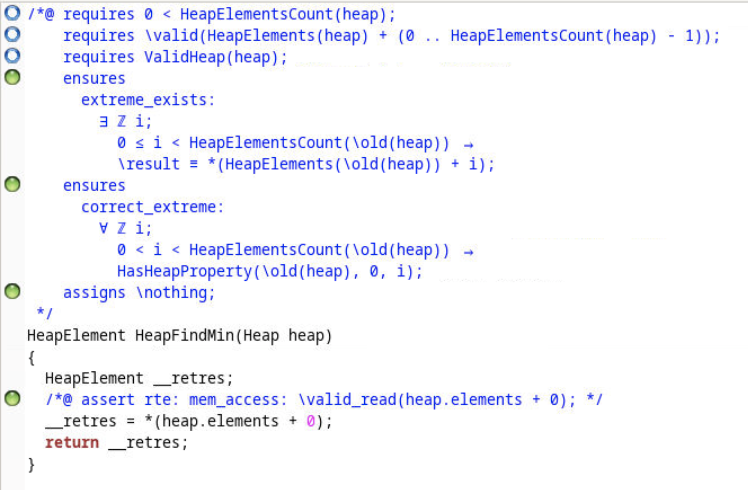
\includegraphics[width=10cm]{images/frama-c-HeapFindMin}
	\caption{Úspešné dokončení důkazu hledání minimálního prvku v prostředí Frama-C}
	\label{img:F-C-HeapFindMin}
\end{figure}

Na obrázku \ref{img:F-C-HeapFindMin} je vidět úspěšně dokončený důkaz korektnosti hledání minimálního prvku v~haldě.

Ostatní funkce a anotace v implementaci binární haldy nevyužívají axiomy a lze dokázat jejich korektnost pomocí nástrojů \mbox{\textit{Alt-Ergo}} nebo \textit{CVC4}.

\section{Probublání prvku nahoru}
\label{subsec:HeapBubbleUp}

Probublání prvku haldy směrem nahoru (ke kořeni) je operace nad haldou, která dokáže v čase $\mathcal{O}(\log(n))$ opravit haldové uspořádání za předpokladu, že se snížila pouze hodnota prvku uloženého ve vrcholu, který má být probublán.

Algoritmus předpokládá, že haldové uspořádání lze porušit pouze mezi jednou dvojicí prvků ve vrcholech $u$ a $v$, kde $u$ je rodičovský vrchol a $v$ je jeho potomek. Tedy v celé haldě s výjimkou této dvojice musí platit haldové uspořádání. V této dvojici může platit, že prvek ve vrcholu $v$~má menší hodnotu než prvek ve vrcholu~$u$. Dále se předpokládá, že tento algoritmus bude proveden po zmenšení hodnoty některého prvku haldy nebo po vložení nového prvku do haldy. V~obou případech je potřeba daný prvek probublat nahoru do správné pozice v haldě. Pokud by se hodnota prvku zvýšila, měl by být aplikován algoritmus probublání dolů, o kterém pojednává sekce \ref{subsec:HeapBubbleDown}.

\begin{listing}[H]
	\caption{Probublání prvku nahoru}
	\label{list:HeapBubbleUp}
	\begin{minted}{c}
void HeapBubbleUp(Heap heap, int index) {
  int parent;

  while (HeapHasParent(heap, index)) {
    parent = HeapParent(index);

    if (HeapElementValue(heap, parent) <= HeapElementValue(heap, index)) {
      break;
    }

    HeapSwap(heap, index, parent);

    index = parent;
  }
}
	\end{minted}
\end{listing}

Pro důkaz korektnosti algoritmu probublání nahoru, zobrazeného ve výpisu kódu \ref{list:HeapBubbleUp}, jsou použity \textit{řezy} haldou. Tyto řezy slouží pro rozdělení grafu haldy na dva podgrafy, ve kterých platí haldové uspořádání. Řezy dohromady tvoří původní graf haldy bez jedné problematické hrany $(u, v)$, na které nemusí platit haldové uspořádání.

Rozdělení haldy pro operaci probublání nahoru by mohlo vypadat podobně jak znázorňuje obrázek \ref{img:heap-intuitive-cut}. Tento přístup ale není vhodný pro algoritmické zpracování a dokazovaní, jelikož se toto rozdělení složitě popisuje. Zavedeme proto horní a spodní řez haldy pomocí potomka, které pracují s indexy jednotlivých vrcholů haldy reprezentované polem.

\begin{figure}[H]
	\centering
	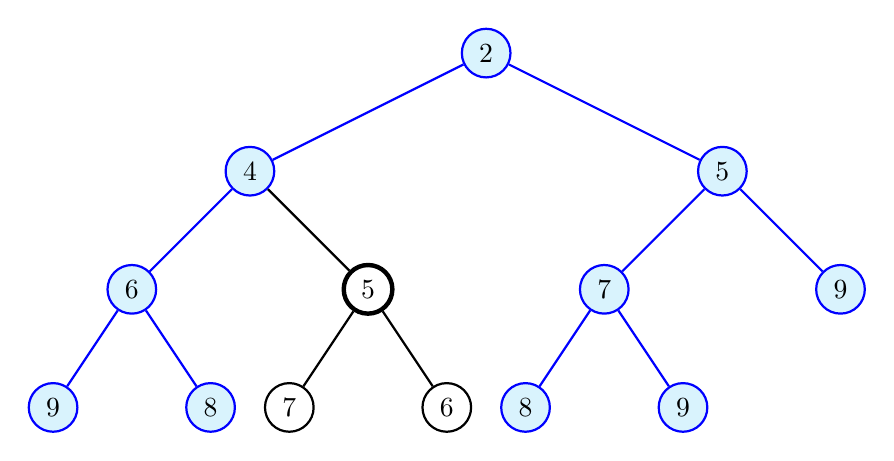
\begin{tikzpicture}[level/.style={sibling distance=60mm/#1}]
		\node [circle,thick,draw=blue,fill=cyan!15] (0) {2}
		child[thick,draw=blue] { node [circle,draw,fill=cyan!15] (1) {4}
			child { node [circle,draw,fill=cyan!15] (3) {6}
				child { node [circle,draw,fill=cyan!15] (7) {9} }
				child { node [circle,draw,fill=cyan!15] (8) {8} }
			}
			child[draw=black] { node [circle,draw,ultra thick] (4) {5}
				child { node [circle,draw] (9) {7} }
				child { node [circle,draw] (10) {6} }
			}
		}
		child[thick,draw=blue] { node [circle,draw,fill=cyan!15] (2) {5}
			child { node [circle,draw,fill=cyan!15] (5) {7}
				child { node [circle,draw,fill=cyan!15] (11) {8} }
				child { node [circle,draw,fill=cyan!15] (12) {9} }
			}
			child { node [circle,draw,fill=cyan!15] (6) {9} }
		};
	\end{tikzpicture}
	\caption{Ukázka intuitivního řezu haldy}
	\label{img:heap-intuitive-cut}
\end{figure}

\begin{definition}[Vrchní řez haldy pomocí potomka]
	Mějme graf $G = (V, E)$ reprezentující binární haldu a~$i \in \mathbb{N}$.
	Vrchním řezem haldy pomocí potomka nazveme graf $G' = (V', E')$, kde
	\begin{enumerate}
	  \item[] $V' = \{ v: v \in V \land \Index(v) < i \}$
	  \item[] $E' = \{ (u, v): (u, v) \in E \land u \in V' \land v \in V' \}$.
	\end{enumerate}
\end{definition}

\pagebreak

Obrázek \ref{img:heap-upper-child-cut} zobrazuje ukázku vrchního řezu haldy pomocí potomka pro index $4$ na kterém se aktuálně nachází prvek s hodnotou 5.

\begin{figure}[H]
	\centering
	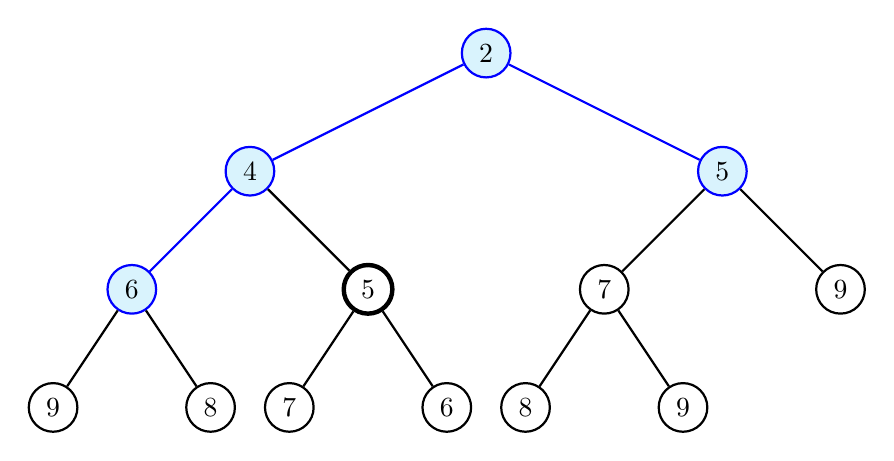
\begin{tikzpicture}[level/.style={sibling distance=60mm/#1}]
		\node [circle,thick,draw=blue,fill=cyan!15] (0) {2}
		child[thick,draw=blue] { node [circle,draw,fill=cyan!15] (1) {4}
			child { node [circle,draw,fill=cyan!15] (3) {6}
				child[draw=black] { node [circle,draw] (7) {9} }
				child[draw=black] { node [circle,draw] (8) {8} }
			}
			child[draw=black] { node [circle,draw,ultra thick] (4) {5}
				child { node [circle,draw] (9) {7} }
				child { node [circle,draw] (10) {6} }
			}
		}
		child[thick,draw=blue] { node [circle,draw,fill=cyan!15] (2) {5}
			child[draw=black] { node [circle,draw] (5) {7}
				child { node [circle,draw] (11) {8} }
				child { node [circle,draw] (12) {9} }
			}
			child[draw=black] {node [circle,draw] (6) {9} }
		};
	\end{tikzpicture}
	\caption{Ukázka vrchního řezu haldy pomocí potomka}
	\label{img:heap-upper-child-cut}
\end{figure}

\begin{remark}
	V grafu vrchního řezu haldy pomocí potomka platí haldové uspořádání.
\end{remark}

ACSL predikát zobrazený ve výpisu kódu \ref{acsl:HeapUpperChildCut} popisuje vrchní řez haldy pomocí potomka. Tento predikát nevytváří nový podgraf s~výše definovanými vlastnostmi, ale pouze ověřuje, že daná část (podgraf) haldy splňuje haldové uspořádání. Takto vytvořený predikát je následně použit v~kontraktu funkce jako jedna ze vstupních podmínek algoritmu probublání nahoru a je také použit jako invariant cyklu. Predikát je tedy platný při volání funkce, po každém kroku cyklu a je také platný na konci vykonávání funkce. Tato induktivní vlastnost následně napomáhá při dokončení důkazu korektnosti algoritmu. Nemusí ale platit, že graf vrchního řezu haldy pomocí potomka je na konci vykonávání funkce prázdný. Tato situace nastává pouze v případě, když je problematický prvek probublán až do kořene haldy.

\begin{listing}[H]
	\caption{Predikát validního vrchního řezu v haldě pomocí potomka}
	\label{acsl:HeapUpperChildCut}
	\begin{minted}{c}
/*@
  predicate HeapUpperChildCut(Heap heap, integer index) =
    \forall integer ancestor, descendant;
      0 <= ancestor < descendant < HeapElementsCount(heap)
      && descendant < index
      && IsParent(ancestor, descendant) ==>
        HasHeapProperty(heap, ancestor, descendant);
*/
	\end{minted}
\end{listing}

\begin{definition}[Spodní řez haldy pomocí potomka]
	Mějme graf $G = (V, E)$ reprezentující binární haldu a~$i \in \mathbb{N}$.
	Spodním řezem haldy pomocí potomka nazveme graf $G' = (V', E')$, kde
	\begin{enumerate}
	  \item[] $V' = \{ v: v \in V \land \Index(v) > i \} \cup \{ \Parent(v): v \in V \land \Index(v) > i \}$
	  \item[] $E' = \{ (u, v): (u, v) \in E \land u \in V' \land v \in V' \}$.
	\end{enumerate}
\end{definition}

\pagebreak

Obrázek \ref{img:heap-lower-child-cut} zobrazuje ukázku spodního řezu haldy pomocí potomka pro index $4$ na kterém se nachází prvek s hodnotou 5.

\begin{figure}[H]
	\centering
	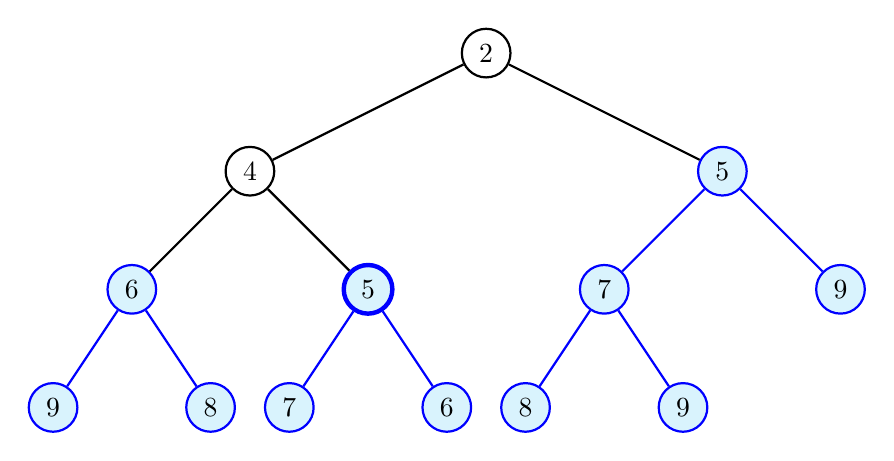
\begin{tikzpicture}[level/.style={sibling distance=60mm/#1}]
		\node [circle,thick,draw] (0) {2}
		child[thick] { node [circle,draw] (1) {4}
			child { node [circle,draw=blue,fill=cyan!15] (3) {6}
				child[draw=blue] { node [circle,draw,fill=cyan!15] (7) {9} }
				child[draw=blue] { node [circle,draw,fill=cyan!15] (8) {8} }
			}
			child { node [circle,draw=blue,fill=cyan!15,ultra thick] (4) {5}
				child[draw=blue] { node [circle,draw,fill=cyan!15] (9) {7} }
				child[draw=blue] { node [circle,draw,fill=cyan!15] (10) {6} }
			}
		}
		child[thick] { node [circle,draw=blue,fill=cyan!15] (2) {5}
			child[draw=blue] { node [circle,draw,fill=cyan!15] (5) {7}
				child { node [circle,draw,fill=cyan!15] (11) {8} }
				child { node [circle,draw,fill=cyan!15] (12) {9} }
			}
			child[draw=blue] {node [circle,draw,fill=cyan!15] (6) {9} }
		};
	\end{tikzpicture}
	\caption{Ukázka spodního řezu haldy pomocí potomka}
	\label{img:heap-lower-child-cut}
\end{figure}

\begin{remark}
	V grafu spodního řezu haldy pomocí potomka platí haldové uspořádání.
\end{remark}

ACSL predikát zobrazený ve výpisu kódu \ref{acsl:HeapLowerChildCut} popisuje spodní řez haldy pomocí potomka. Tento predikát je velmi podobný predikátu vrchního řezu haldy pomocí potomka. Pokrývá ale vrcholy haldy s indexem větším než problematický vrchol a jejich rodičovské vrcholy. Nemusí ale platit, že graf spodního řezu haldy pomocí potomka na konci vykonávání funkce obsahuje celou původní haldu. Tato situace nastává pouze v případě, když je problematický prvek probublán až do kořene haldy.

\begin{listing}[H]
	\caption{Predikát validního spodního řezu v haldě pomocí potomka}
	\label{acsl:HeapLowerChildCut}
	\begin{minted}{c}
/*@
  predicate HeapLowerChildCut(Heap heap, integer index) =
    \forall integer ancestor, descendant;
      0 <= ancestor < descendant < HeapElementsCount(heap)
      && index < descendant
      && IsParent(ancestor, descendant) ==>
        HasHeapProperty(heap, ancestor, descendant);
*/
	\end{minted}
\end{listing}

ACSL predikát spodního řezu haldy pomocí potomka správně odděluje vrcholy haldy, které mají index větší než problematický vrchol. Zároveň ale neomezuje indexy rodičovských vrcholů. Proto je ve spodním řezu pomocí potomka správně obsažen problematický vrchol jako rodičovský vrchol a také některé rodičovské vrcholy, které mají menší index než problematický vrchol. Hrana mezi problematickým vrcholem a jeho rodičovským vrcholem zde správně není obsažena.

Poslední nutnou vlastností pro úspěšné dokončení důkazu je tranzitivní haldové uspořádání mezi vrchním a spodním řezem haldy. Tato vlastnost je automaticky splněna pro všechny hrany v~haldě s výjimkou hrany, na které leží problematický vrchol v roli potomka. Proto je do kódu zavedena vstupní podmínka a invariantu cyklu, které kontrolují, zda platí haldové uspořádání pro rodičovský vrchol problematického vrcholu a jednotlivé potomky problematického vrcholu.

Predikáty tranzitivního haldového uspořádání zobrazené ve výpisu kódu \ref{acsl:HeapCutHeapPropertyTransitive} umožňují probublávat problematický vrchol nahoru. Zaručují totiž, že rodičovský prvek, který s problematickým vrcholem vyměníme, bude po provedení výměny splňovat haldové uspořádání se svými novými potomky.

\begin{listing}[H]
	\caption{Predikáty tranzitivního haldového uspořádání mezi řezy haldou}
	\label{acsl:HeapCutHeapPropertyTransitive}
	\begin{minted}{c}
/*@
  predicate HeapCutHeapPropertyLeftChild(Heap heap, integer index) = 
    HeapHasParent(heap, index)
    && HeapHasLeftChild(heap, index) ==>
      HasHeapProperty(heap, Parent(index), LeftChild(index));

  predicate HeapCutHeapPropertyRightChild(Heap heap, integer index) =
    HeapHasParent(heap, index)
    && HeapHasRightChild(heap, index) ==>
      HasHeapProperty(heap, Parent(index), RightChild(index));
*/
	\end{minted}
\end{listing}

Platnost těchto čtyř invariantů cyklu dokazuje, že algoritmus probublání nahoru vždy vytvoří maximálně jednu novou problematickou dvojici vrcholů. Haldové uspořádání mezi touto dvojicí vrcholů je opraveno probubláním prvku na správnou pozici v haldě.

V prostředí Frama-c lze formálně dokázat korektnost celé funkce probublání prvku nahoru. Jelikož platí výše zmíněné čtyři invarianty cyklu, po ukončení cyklu se halda nachází v jednom z těchto stavů:

\begin{enumerate}
  \item problematický prvek probublal až do kořene haldy,
  \item problematický prvek nemohl dále probublat, tudíž je na správné pozici v haldě.
\end{enumerate}

Spojením platnosti invariantů cyklu a znalostí o aktuálně opravené hraně dává dostatečné důkazy pro verifikační prostředí, že pro každou hranu $(u, v)$ dané haldy, kde $u$ je rodičovský vrchol $v$, platí haldové uspořádání. Úspěšně dokončený důkaz korektnosti funkce probublání nahoru je zobrazen na obrázku \ref{img:F-C-HeapBubbleUp}.

\begin{figure}[H]
	\centering
	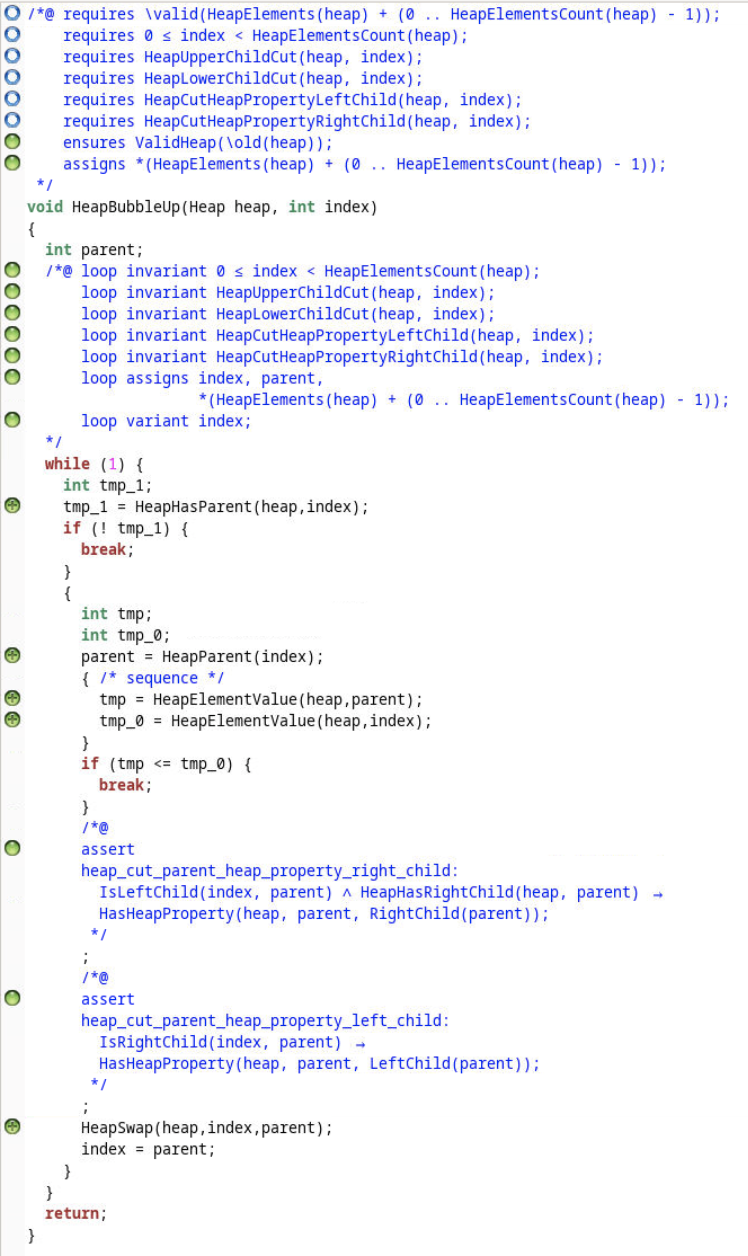
\includegraphics[width=10cm]{images/frama-c-HeapBubbleUp}
	\caption{Úspešné dokončení důkazu probublání nahoru v prostředí Frama-C}
	\label{img:F-C-HeapBubbleUp}
\end{figure}

\section{Vložení prvku}
\label{subsec:HeapInsert}

Vložení prvku do haldy je operace nad haldou, která v čase $\mathcal{O}(1)$ vloží nový prvek do haldy a~následně v~čase $\mathcal{O}(\log(n))$ tento prvek umístí na správnou pozici v haldě. Celková asymptotická časová složitost je tedy $\mathcal{O}(\log(n))$.

Algoritmus přidává nový vrchol do nejspodnější hladiny haldy tak, aby byl udržen tvar haldy. Pro takto vložený vrchol nemusí platit haldové uspořádání s jeho rodičovským vrcholem. Mohlo se stát, že hodnota prvku v nově přidaném vrcholu má menší hodnotou než hodnota prvku v~jeho rodičovském vrcholu. Proto je nutné provést probublání nahoru, o kterém pojednává sekce \ref{subsec:HeapBubbleUp}.

Algoritmus probublání nahoru má tři vstupní podmínky. V haldě musí platit predikát o~horním řezu haldy pomocí potomka, který v případě přidání nového vrcholu platí. Před přidáním vrcholu byla halda validní a platilo v ní haldové uspořádání. Nový prvek je vložen na nový největší index v haldě. Tedy pro tento nový index platí vrchní řez haldou pomocí potomka, protože tento řez popisuje původní haldu, ve které platilo haldové uspořádání. Spodní řez haldy pomocí potomka také platí, protože se jedná o prázdný graf. Tranzitivní haldové uspořádání u aktuálně přidaného vrcholu také platí, protože tento vrchol nemá žádné potomky.

\begin{figure}[H]
	\centering
	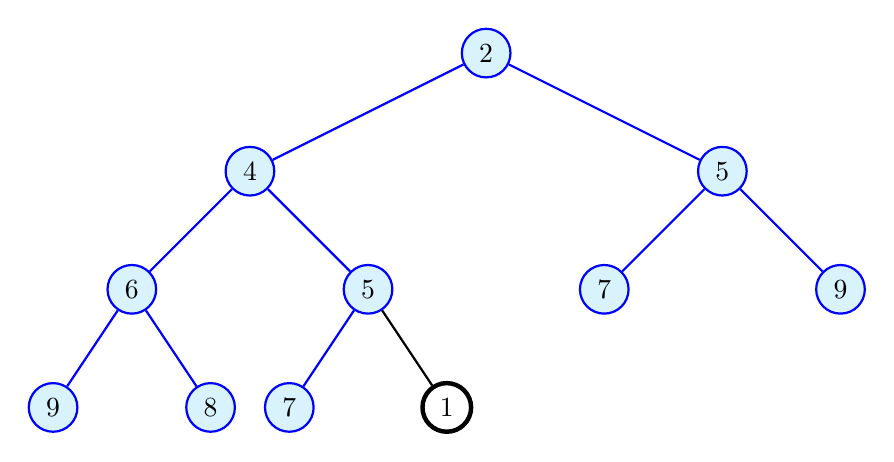
\begin{tikzpicture}[level/.style={sibling distance=60mm/#1}]
		\node [circle,thick,draw=blue,fill=cyan!15] (0) {2}
		child[thick,draw=blue] { node [circle,draw,fill=cyan!15] (1) {4}
			child { node [circle,draw,fill=cyan!15] (3) {6}
				child { node [circle,draw,fill=cyan!15] (7) {9} }
				child { node [circle,draw,fill=cyan!15] (8) {8} }
			}
			child { node [circle,draw,,fill=cyan!15] (4) {5}
				child { node [circle,draw,fill=cyan!15] (9) {7} }
				child[draw=black] { node [circle,draw,ultra thick] (10) {1} }
			}
		}
		child[thick,draw=blue] { node [circle,draw,fill=cyan!15] (2) {5}
			child { node [circle,draw,fill=cyan!15] (5) {7} }
			child { node [circle,draw,fill=cyan!15] (6) {9} }
		};
	\end{tikzpicture}
	\caption{Ukázka vrchního řezu haldy pomocí potomka při přidání vrcholu}
	\label{img:heap-insert-heap-upper-child-cut}
\end{figure}

Na obrázku \ref{img:heap-insert-heap-upper-child-cut} je zobrazeno přidání nového vrcholu do haldy a je zvýrazněn horní řez haldy pomocí potomka.

Algoritmus probublání nahoru tento nový vrchol vymění s jeho rodičovským vrcholem, protože hodnota prvku v nově přidaném vrcholu má menší hodnotu než prvek v jeho rodičovském vrcholu. Tímto prvním krokem algoritmu se nově přidaný vrchol dostal výše v haldě, ale stále platí všechny čtyři invarianty cyklu. Horní řez haldy pomocí potomka se pouze zmenšil a spodní řez haldy pomocí potomka se zvětšil o vrcholy, které se v předchozím kroku vyskytovaly v horním řezu pomocí potomka a také o vrchol původního rodiče nového vrcholu. Tranzitivní haldové uspořádání začíná platit mezi rodičovským prvkem aktuálně probublaného vrcholu a jeho potomky.

Algoritmem probublání se nový vrchol dostane do správné pozice a ve výsledné haldě, o jeden vrchol větší, je opraveno haldové uspořádání.

\begin{listing}[H]
	\caption{Vložení prvku}
	\label{list:HeapInsert}
	\begin{minted}{c}
/*@
    requires 0 <= HeapElementsCount(heap) < HeapElementsCapacity(heap);
    requires \valid(HeapElements(heap) + (0 .. HeapElementsCapacity(heap) - 1));
    requires ValidHeap(heap);
    requires correctly_indexed:
    	HeapElementIndex(element) == HeapElementsCount(heap);

    assigns HeapElements(heap)[0..HeapElementsCount(heap)];
    
    ensures count_increase: 
    	HeapElementsCount(\result) == HeapElementsCount(heap) + 1;
    ensures ValidHeap(\result);
*/
Heap HeapInsert(Heap heap, HeapElement element) {
  int index = heap.elementsCount;

  heap.elements[index] = element;
  heap.elementsCount++;

  HeapBubbleUp(heap, index);

  return heap;
}
	\end{minted}
\end{listing}

Výpis kódu \ref{list:HeapInsert} zobrazuje funkci pro přidání nového prvku do haldy společně s kontraktem této funkce. ACSL anotace funkce probublání nahoru zajišťují, že po dokončení probublání nahoru je předaná halda opravená a platí v ní haldové uspořádání. Jelikož je volání funkce probublání nahoru poslední akcí funkce vložení prvku, lze ujištění validnosti haldy vložit také do kontraktu funkce vkládání prvku. Tímto je zaručena korektnost funkce vkládání prvku do haldy. Obrázek~\ref{img:F-C-HeapInsert} zobrazuje úspěšně dokončený důkaz korektnosti funkce v prostředí Frama-C.

\begin{figure}[H]
	\centering
	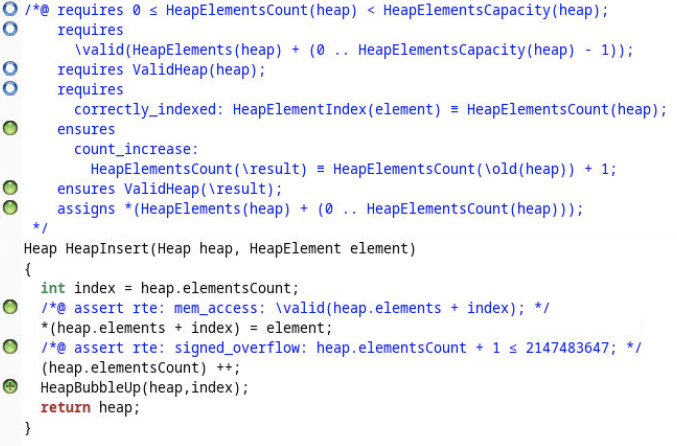
\includegraphics[width=10cm]{images/frama-c-HeapInsert}
	\caption{Úspešné dokončení důkazu vložení prvku do haldy v prostředí Frama-C}
	\label{img:F-C-HeapInsert}
\end{figure}


\section{Probublání prvku dolů}
\label{subsec:HeapBubbleDown}

Probublání prvku haldy směrem dolů (od kořene) je operace nad haldou, která dokáže v čase $\mathcal{O}(\log(n))$ opravit haldové uspořádání za předpokladu, že se zvýšila pouze hodnota prvku uloženého ve vrcholu, který má být probublán.

Algoritmus předpokládá, že haldové uspořádání lze porušit maximálně u dvou dvojic vrcholů $u$ a $v$ nebo $u$ a $w$, kde $u$ je rodičovský vrchol vrcholů $v$ a $w$. Tedy v celé haldě s výjimkou těchto dvou dvojic vrcholů musí platit haldové uspořádání. V těchto dvojicích může platit, že prvek uložený ve vrcholu $u$~má větší hodnotu než některý prvek uložený ve vrcholech $v$ nebo $w$. Může nastat situace, kdy prvek ve vrcholu $u$~má větší hodnotu než oba prvky ve vrcholech $v$ a $w$. Dále se předpokládá, že tento algoritmus bude proveden po zvětšení hodnoty některého prvku haldy nebo při vytváření haldy. V obou případech je potřeba tento vrchol probublat dolů do správné pozice v haldě. Pokud by se hodnota snížila, měl by být aplikován algoritmus probublání nahoru, o kterém pojednává sekce \ref{subsec:HeapBubbleUp}.


\begin{listing}[H]
	\caption{Probublání prvku dolů}
	\label{list:HeapBubbleDown}
	\begin{minted}{c}
void HeapBubbleDown(Heap heap, int index) {
    int child;

    while (HeapHasChild(heap, index)) {
        child = HeapLowerChild(heap, index);

        if (HeapElementValue(heap, index) <= HeapElementValue(heap, child)) {
            break;
        }

        HeapSwap(heap, index, child);

        index = child;
    }
}
	\end{minted}
\end{listing}

Pro důkaz korektnosti algoritmu probublání dolů, zobrazeného ve výpisu kódu \ref{list:HeapBubbleDown}, jsou použity \textit{řezy} haldou, podobné řezům v~důkazu korektnosti algoritmu probublání nahoru, které byly představeny v sekci \ref{subsec:HeapBubbleUp}. Řezy haldou pro důkaz probublání dolů jsou mírně odlišné od řezů v~důkazu korektnosti algoritmu probublání nahoru. Řezy haldou pomocí rodiče totiž povolují až dvě problematické hrany v haldě.

\begin{definition}[Vrchní řez haldy pomocí rodiče]
	Mějme graf $G = (V, E)$ reprezentující binární haldu a~$i \in \mathbb{N}$.
	Vrchním řezem haldy pomocí rodiče nazveme graf $G' = (V', E')$, kde
	\begin{enumerate}
	  \item[] $V' = \{ v: v \in V \land \Index(v) < i \} \cup \{ \LeftChild(v): v \in V \land \Index(v) < i \} \cup \{ \RightChild(v): v \in V \land \Index(v) < i \}$
	  \item[] $E' = \{ (u, v): (u, v) \in E \land u \in V' \land v \in V' \}$.
	\end{enumerate}
\end{definition}

\pagebreak

Obrázek \ref{img:heap-upper-parent-cut} zobrazuje ukázku vrchního řezu haldy pomocí rodiče pro index 3 na kterém se nachází prvek s hodnotou 6.

\begin{figure}[H]
	\centering
	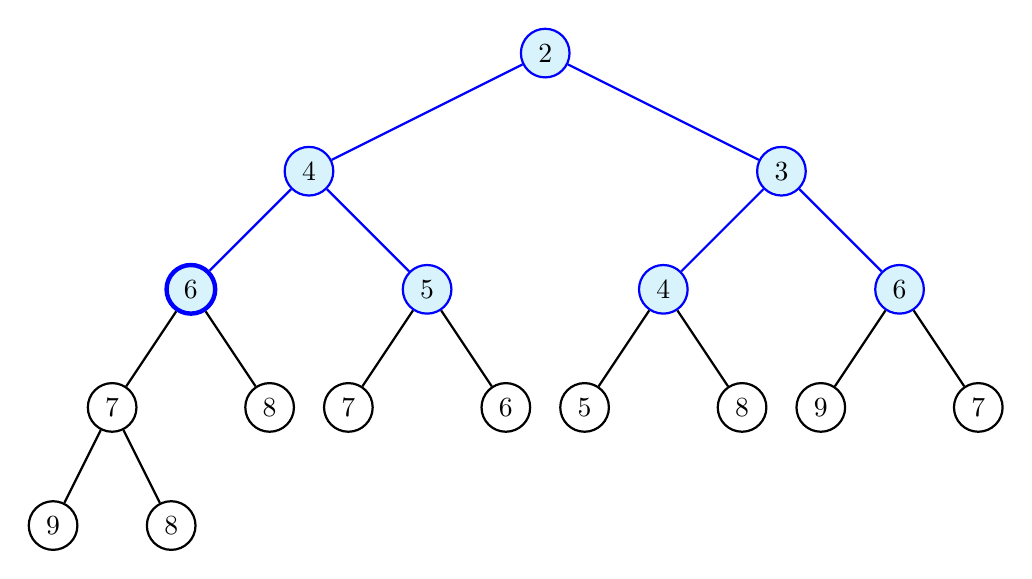
\begin{tikzpicture}[level/.style={sibling distance=60mm/#1}]
		\node [circle,thick,draw=blue,fill=cyan!15] (0) {2}
		child[thick,draw=blue] { node [circle,draw,fill=cyan!15] (1) {4}
			child { node [circle,draw,ultra thick,fill=cyan!15] (3) {6}
				child[draw=black] { node [circle,draw] (7) {7} 
					child { node [circle,draw] (15) {9} }
					child { node [circle,draw] (16) {8} }				
				}
				child[draw=black] { node [circle,draw] (8) {8} }
			}
			child { node [circle,draw,fill=cyan!15] (4) {5}
				child[draw=black] { node [circle,draw] (9) {7} }
				child[draw=black] { node [circle,draw] (10) {6} }
			}
		}
		child[thick,draw=blue] { node [circle,draw,fill=cyan!15] (2) {3}
			child { node [circle,draw,fill=cyan!15] (5) {4}
				child[draw=black] { node [circle,draw] (11) {5} }
				child[draw=black] { node [circle,draw] (12) {8} }
			}
			child { node [circle,draw,fill=cyan!15] (7) {6}
				child[draw=black] { node [circle,draw] (13) {9} }
				child[draw=black] { node [circle,draw] (14) {7} }
			}
		};
	\end{tikzpicture}
	\caption{Ukázka vrchního řezu haldy pomocí rodiče}
	\label{img:heap-upper-parent-cut}
\end{figure}

\begin{remark}
	V grafu vrchního řezu haldy pomocí rodiče platí haldové uspořádání.
\end{remark}

ACSL predikát zobrazený ve výpisu kódu \ref{acsl:HeapUpperParentCut} popisuje vrchní řez haldy pomocí rodiče. Tento predikát nevytváří nový podgraf s~výše definovanými vlastnostmi, ale pouze ověřuje, že daná část (podgraf) haldy splňuje haldové uspořádání. Takto vytvořený predikát je následně použit v~kontraktu funkce jako jedna ze vstupních podmínek algoritmu probublání dolů a je také použit jako invariant cyklu. Predikát je tedy platný při volání funkce, po každém kroku cyklu a je také platný na konci vykonávání funkce. Tato induktivní vlastnost následně napomáhá při dokončení důkazu korektnosti algoritmu. Nemusí ale platit, že graf vrchního řezu haldy pomocí rodiče na konci vykonávání funkce obsahuje celou původní haldu. Tato situace nastává pouze v případě, když je problematický prvek probublán do vrcholu s maximálním indexem v haldě.

\begin{listing}[H]
	\caption{Predikát validního vrchního řezu v haldě pomocí rodiče}
	\label{acsl:HeapUpperParentCut}
	\begin{minted}{c}
/*@
  predicate HeapUpperParentCut(Heap heap, integer index) =
    \forall integer ancestor, descendant;
      0 <= ancestor < index
      && ancestor < descendant < HeapElementsCount(heap)
      && IsParent(ancestor, descendant) ==>
        HasHeapProperty(heap, ancestor, descendant);
*/
	\end{minted}
\end{listing}

\begin{definition}[Spodní řez haldy pomocí rodiče]
	Mějme graf $G = (V, E)$ reprezentující binární haldu a~$i \in \mathbb{N}$.
	Spodním řezem haldy pomocí rodiče nazveme graf $G' = (V', E')$, kde
	\begin{enumerate}
	  \item[] $V' = \{ v: v \in V \land \Index(v) > i \}$
	  \item[] $E' = \{ (u, v): (u, v) \in E \land u \in V' \land v \in V' \}$.
	\end{enumerate}
\end{definition}

\pagebreak

Obrázek \ref{img:heap-lower-parent-cut} zobrazuje ukázku spodního řezu haldy pomocí rodiče pro index 3 na kterém se nachází prvek s hodnotou 6.

\begin{figure}[H]
	\centering
	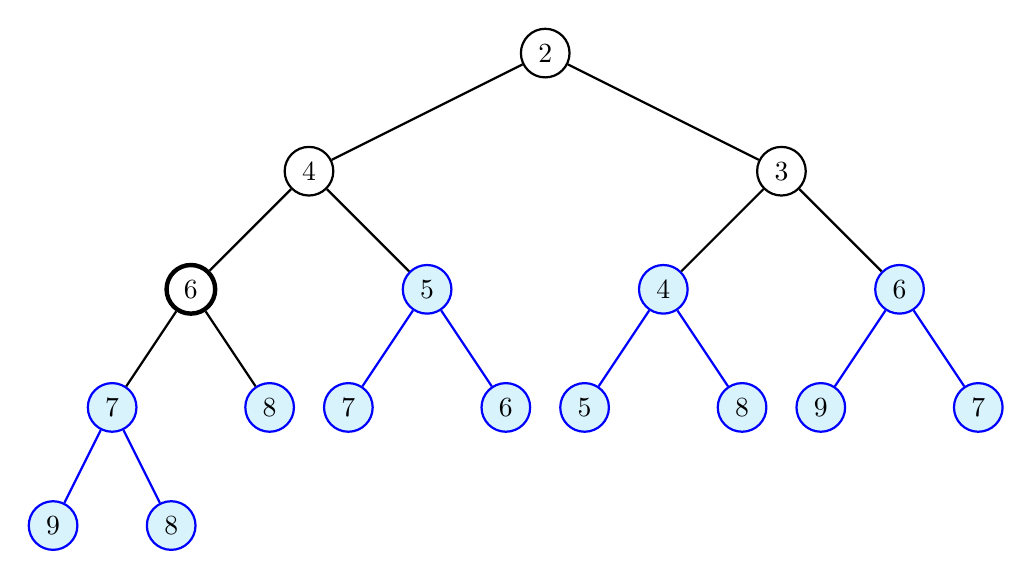
\begin{tikzpicture}[level/.style={sibling distance=60mm/#1}]
		\node [circle,draw,thick] (0) {2}
		child[thick] { node [circle,draw] (1) {4}
			child { node [circle,draw,ultra thick] (3) {6}
				child { node [circle,draw=blue,fill=cyan!15] (7) {7} 
					child[draw=blue] { node [circle,draw,fill=cyan!15] (15) {9} }
					child[draw=blue] { node [circle,draw,fill=cyan!15] (16) {8} }				
				}
				child { node [circle,draw=blue,fill=cyan!15] (8) {8} }
			}
			child { node [circle,draw=blue,fill=cyan!15] (4) {5}
				child[draw=blue] { node [circle,draw,fill=cyan!15] (9) {7} }
				child[draw=blue] { node [circle,draw,fill=cyan!15] (10) {6} }
			}
		}
		child[thick] { node [circle,draw] (2) {3}
			child { node [circle,draw=blue,fill=cyan!15] (5) {4}
				child[draw=blue] { node [circle,draw,fill=cyan!15] (11) {5} }
				child[draw=blue] { node [circle,draw,fill=cyan!15] (12) {8} }
			}
			child { node [circle,draw=blue,fill=cyan!15] (7) {6}
				child[draw=blue] { node [circle,draw,fill=cyan!15] (13) {9} }
				child[draw=blue] { node [circle,draw,fill=cyan!15] (14) {7} }
			}
		};
	\end{tikzpicture}
	\caption{Ukázka spodního řezu haldy pomocí rodiče}
	\label{img:heap-lower-parent-cut}
\end{figure}

\begin{remark}
	V grafu spodního řezu haldy pomocí rodiče platí haldové uspořádání.
\end{remark}

ACSL predikát zobrazený ve výpisu kódu \ref{acsl:HeapLowerParentCut} popisuje spodní řez haldy pomocí rodiče. Tento predikát je velmi podobný predikátu vrchního řezu haldy pomocí rodiče. Pokrývá ale vrcholy haldy s indexem větším než problematický vrchol. Nemusí ale platit, že graf spodního řezu haldy pomocí rodiče je na konci vykonávání funkce prázdný. Tato situace nastává pouze v případě, když je problematický prvek probublán do vrcholu s maximálním indexem v haldě.

\begin{listing}[H]
	\caption{Predikát validního spodního řezu v haldě pomocí rodiče}
	\label{acsl:HeapLowerParentCut}
	\begin{minted}{c}
/*@
  predicate HeapLowerParentCut(Heap heap, integer index) =
    \forall integer ancestor, descendant;
      index < ancestor < HeapElementsCount(heap)
      && ancestor < descendant < HeapElementsCount(heap)
      && IsParent(ancestor, descendant) ==>
        HasHeapProperty(heap, ancestor, descendant);
*/
	\end{minted}
\end{listing}

Algoritmus probublání dolů je v binární haldě aplikován po zvýšení hodnoty některého prvku nebo při rychlé konstrukci haldy, o které pojednává sekce \ref{subsec:HeapBuild}. Při zvýšení hodnoty prvku haldy můžeme využít horní a dolní řez haldou pomocí rodiče a pomocí invariantů cyklu formálně dokázat korektnosti algoritmu.

Problém představuje algoritmus rychlé konstrukce haldy. Tento algoritmu postupně probublává dolů rodičovské vrcholy od vrcholu s největším indexem až po index kořene haldy. Při tomto způsobu konstrukce je haldové uspořádání zaručeno pouze v dolním řezu haldy pomocí rodiče.

Kontrakt funkce probublání dolů rozlišuje základní a rozšířené vstupní podmínky. Základní podmínky musejí být splněny při všech voláních funkce probublání dolů.

Pokud volající splňuje pouze základní vstupní podmínky kontraktu funkce probublání dolů, tak funkce zajišťuje pouze částečné opravení haldy. Základní podmínky požadují platný predikát o~spodním řezu haldy pomocí rodiče. Pokud je tato základní podmínka splněna, kontrakt funkce volajícího ujišťuje, že ve výsledné haldě bude platit původní spodní řez haldy pomocí rodiče rozšířený o~právě probublávaný vrchol. Tato vlastnost je vhodná při postupné konstrukci haldy, ve které se halda konstruuje postupným probublávání prvků dolů.

Rozšířené vstupní podmínky požadují platný predikát o~horním řezu haldy pomocí rodiče a~tranzitivitu haldového uspořádání mezi horním a spodním řezem haldy. Za předpokladu splnění rozšířených podmínek kontrakt funkce zajišťuje, že po provedení funkce probublání dolů bude výsledná halda validní a bude v ní platit haldové uspořádání. Tyto rozšířené vstupní podmínky jsou splněny při zvýšení hodnoty prvku v haldě, jelikož zvýšením hodnoty nebylo porušeno haldové uspořádání v horním řezu haldy pomocí rodiče ani ve spodním řezu haldy pomocí rodiče.

Základní i rozšířené výstupní ujištění v kontraktu funkce je možné dokázat najednou pomocí ACSL konstrukce \textit{behavior}, která umožňuje některé invarianty cyklu dokazovat pouze za předpokladu, že byl algoritmus zavolán s platnými rozšířenými vstupními podmínkami. Obrázek \ref{img:F-C-HeapBubbleDown} zobrazuje úspěšně dokončený důkaz korektnosti funkce probublání dolů v prostředí Frama-C.

\begin{figure}[H]
	\centering
	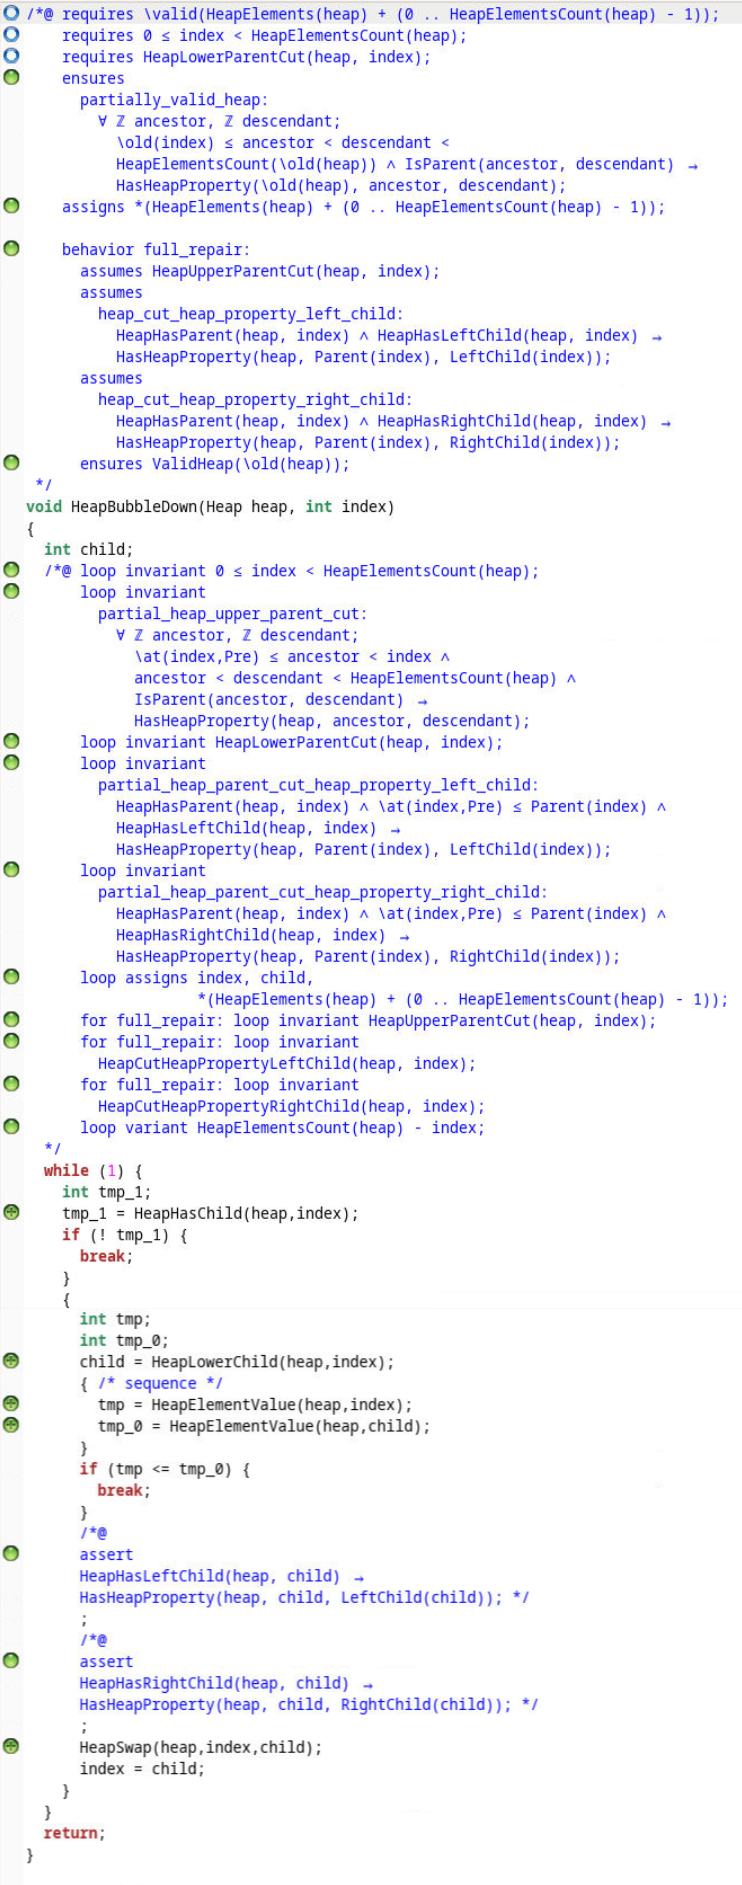
\includegraphics[width=9cm]{images/frama-c-HeapBubbleDown}
	\caption{Úspešné dokončení důkazu probublání dolů v prostředí Frama-C}
	\label{img:F-C-HeapBubbleDown}
\end{figure}

\section{Odstranění minimálního prvku}
\label{subsec:HeapExtractMin}

Kořen binární minimové haldy vždy obsahuje prvek s nejmenší hodnotou. Algoritmy, které haldu využívají jako prioritní frontu, potřebují tento minimální prvek najít a odstranit z fronty. Hledání minimálního prvku zajišťuje algoritmus popsaný v sekci \ref{subsec:HeapFindMin}. Algoritmus odstranění minimálního prvku a důkaz korektnosti je popsán v této sekci.

Odstranění minimálního prvku z haldy je operace nad haldou, která v čase $\mathcal{O}(1)$ odstraní daný prvek z haldy a v čase $\mathcal{O}(\log(n))$ opraví haldové uspořádání. Celková asymptotická časová složitost je tedy $\mathcal{O}(\log(n))$.

Kořen haldy lze odstranit pouze v případě, když je kořen jediným prvkem v haldě. Pokud má kořen nějaké potomky, odstraněním kořene by se porušil tvar haldy.

\begin{remark}
Z haldy lze odstranit prvek s největším indexem bez porušení tvaru haldy.
\end{remark}

Algoritmus v prvním kroku vymění prvek uložený v kořeni haldy s prvkem uloženým ve vrcholu s největším indexem. Ve druhém kroku je vrchol s největším indexem odstraněn z haldy. Poslední krok algoritmu je probublání kořene haldy dolů.

Výměnou prvku v kořeni haldy s prvkem na největším indexu haldy mohlo dojít k porušení haldového uspořádání. Algoritmus probublání dolů je aplikován s rozšířenými vstupními podmínkami, jelikož je splněn horní a dolní řez haldy pomocí rodiče a tranzitivní haldové uspořádání triviálně platí, jelikož kořen nemá žádného rodiče. Horní řez haldy pomocí rodiče je splněn, jelikož se v případě probublání kořene jedná o prázdný graf. Spodní řez haldy pomocí rodiče obsahuje všechny vrcholy bez kořene a všechny hrany, na kterých neleží kořen. Jelikož v původní haldě před výměnou prvku kořene za prvek z vrcholu s největším indexem platilo haldové uspořádání, tak v~podgrafu spodního řezu zmenšené haldy pomocí rodiče musí platit haldové uspořádání.

\begin{figure}[H]
	\centering
	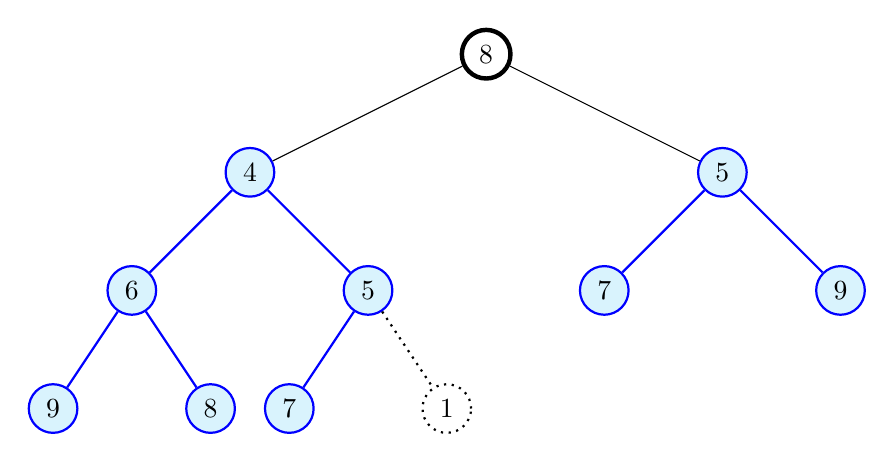
\begin{tikzpicture}[level/.style={sibling distance=60mm/#1}]
		\node [circle,draw,ultra thick] (0) {8}
		child { node [circle,thick,draw=blue,fill=cyan!15] (1) {4}
			child[thick,draw=blue] { node [circle,draw,fill=cyan!15] (3) {6}
				child { node [circle,draw,fill=cyan!15] (7) {9} }
				child { node [circle,draw,fill=cyan!15] (8) {8} }
			}
			child[thick,draw=blue] { node [circle,draw,,fill=cyan!15] (4) {5}
				child { node [circle,draw,fill=cyan!15] (9) {7} }
				child[draw=black,dotted] { node [circle,draw] (10) {1} }
			}
		}
		child { node [circle,thick,draw=blue,fill=cyan!15] (2) {5}
			child[thick,draw=blue] { node [circle,draw,fill=cyan!15] (5) {7} }
			child[thick,draw=blue] { node [circle,draw,fill=cyan!15] (6) {9} }
		};
	\end{tikzpicture}
	\caption{Ukázka spodního řezu haldy pomocí rodiče v průběhu odstraňování minimálního prvku}
	\label{img:heap-extract-min-heap-lower-parent-cut}
\end{figure}

Obrázek \ref{img:heap-extract-min-heap-lower-parent-cut} zobrazuje stav haldy po výměně prvku v kořeni haldy za prvek ve vrcholu s~největším indexem. Tečkovaně je naznačena hrana a vrchol, které se v rámci algoritmu odstraňují a tučně je zvýrazněn nový kořen haldy, který bude v následujícím kroku algoritmu probublán dolů.

\begin{listing}[H]
	\caption{Kód a ACSL anotace odstranění minimálního prvku z haldy}
	\label{code:HeapExtractMin}
	\begin{minted}{c}
/*@
  requires 0 < HeapElementsCount(heap);
  requires \valid(HeapElements(heap) + (0 .. HeapElementsCount(heap) - 1));
  requires ValidHeap(heap);

  assigns HeapElements(heap)[0 .. HeapElementsCount(heap) - 1];

  ensures count_decrease: HeapElementsCount(\result) == HeapElementsCount(heap) - 1;
  ensures ValidHeap(\result);
*/
Heap HeapExtractMin(Heap heap) {
  int last = heap.elementsCount - 1;

  HeapSwap(heap, 0, last);

  heap.elementsCount--;

  if (0 < heap.elementsCount) {
    HeapBubbleDown(heap, 0);
  }

  return heap;
}
	\end{minted}
\end{listing}

Výpis kódu \ref{code:HeapExtractMin} zobrazuje kompletní kód funkce odstranění minimálního prvku z haldy společně s~kontraktem funkce. Vstupní podmínka pro volání této funkce je nenulový počet prvků v haldě a platný predikát o haldovém uspořádání. Výstupní anotace zajišťují, že funkce zmenšuje počet prvků v haldě a také, že ve výsledné zmenšené haldě stále platí haldové uspořádání.

Implementace tohoto algoritmu odhalila, že pro volání probublání dolů kořene je nutné v haldě po odstranění prvku s maximálním indexem alespoň jeden prvek stále mít. Některé pseudokódy tuto podmínku nezohledňují, jelikož se spoléhají na nulový počet kroků cyklu ve funkci probublání dolů. \cite{Pruvodce2017} Z hlediska tvorby formálního důkazu korektnosti tato podmínka musela být zohledněna již ve funkci odstranění minimálního prvku. Tato chyba byla pomocí ACSL odhalena a~bylo ji možné ihned opravit a dokončit důkaz korektnosti. Obrázek \ref{img:F-C-HeapExtractMin} zobrazuje úspěšně dokončený důkaz korektnosti algoritmu odstranění minimálního prvku z haldy.

\begin{figure}[H]
	\centering
	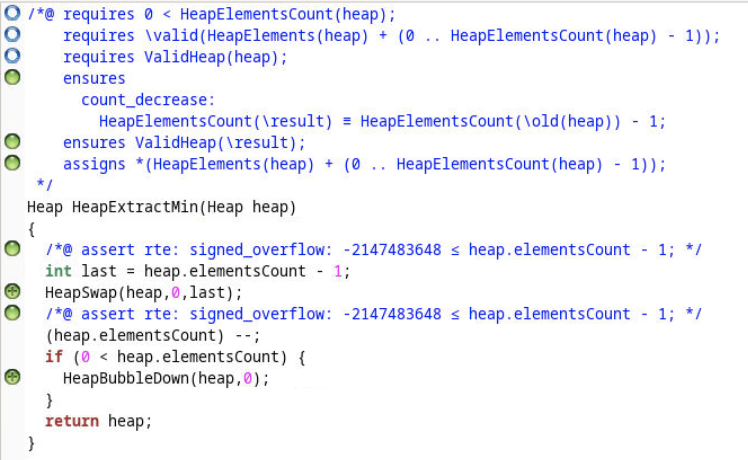
\includegraphics[width=10cm]{images/frama-c-HeapExtractMin}
	\caption{Úspešné dokončení důkazu odstranění minimálního prvku z haldy v prostředí Frama-C}
	\label{img:F-C-HeapExtractMin}
\end{figure}


\section{Změna hodnoty prvku}
\label{subsec:HeapChange}

Algoritmy, které používají binární minimovou haldu, mohou měnit hodnoty jednotlivých prvků v haldě. Jedná se o změnu priority prvku, který lze v haldě jednoznačně identifikovat pomocí indexu pole. Funkce pro změnu hodnoty používá dvě oddělené funkce pro snížení hodnoty prvku a funkci pro zvýšení hodnoty prvku.

\begin{listing}[H]
	\caption{Kód a ACSL anotace změny hodnoty prvku haldy}
	\label{code:HeapChange}
	\begin{minted}{c}
/*@
  requires \valid(HeapElements(heap) + (0 .. HeapElementsCount(heap) - 1));
  requires 0 <= index < HeapElementsCount(heap);
  requires ValidHeap(heap);

  assigns HeapElements(heap)[0 .. HeapElementsCount(heap) - 1];

  ensures value_changed:
    \exists integer i;
      0 <= i < HeapElementsCount(heap) ==>
        HeapElementValue(element) == HeapElementValue(heap, i);
  ensures ValidHeap(heap);
*/
void HeapChange(Heap heap, int index, HeapElement element) {
  if (_HeapElementValue(element) < HeapElementValue(heap, index)) {
    HeapDecrease(heap, index, element);
    return;
  }

  HeapIncrease(heap, index, element);
}
	\end{minted}
\end{listing}

Výpis kódu \ref{code:HeapChange} zobrazuje funkci pro změnu hodnoty prvku v haldě, která pomocí kontroly aktuální hodnoty prvku v haldě a požadované nové hodnotě prvku volá funkci pro zmenšení hodnoty prvku nebo funkci pro zvětšení hodnoty prvku. Obě zmíněné funkce zajišťují změnu hodnoty prvku haldy a následné opravení haldového uspořádání, které se mohlo narušit změnou hodnoty prvku. Jelikož je volání těchto funkcí poslední akce ve funkci pro změnu hodnoty prvku v haldě, lze přidat stejné anotace pro ujištění o změně hodnoty prvku a opravení haldového uspořádání do kontraktu funkce o změně hodnoty prvku v haldě.

\begin{figure}[H]
	\centering
	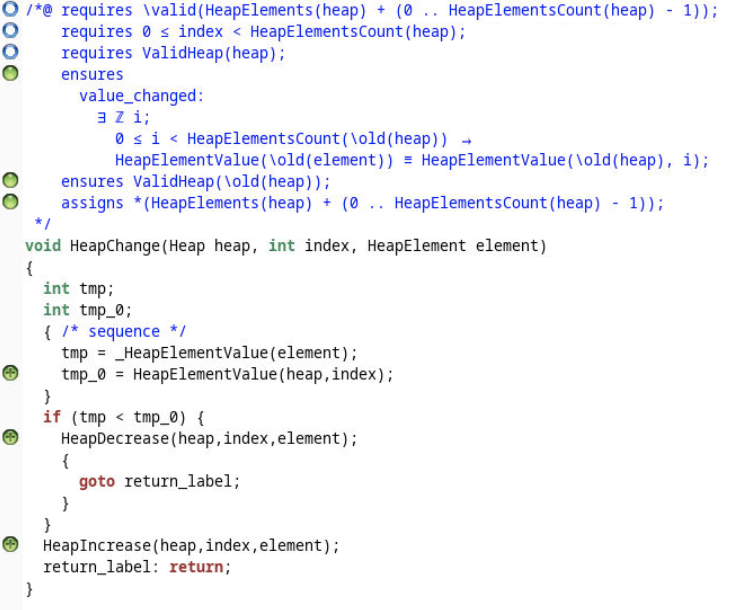
\includegraphics[width=10cm]{images/frama-c-HeapChange}
	\caption{Úspešné dokončení důkazu změny hodnoty prvku haldy v prostředí Frama-C}
	\label{img:F-C-HeapChange}
\end{figure}

Obrázek \ref{img:F-C-HeapChange} zobrazuje úspěšné dokončení důkazu korektnosti funkce pro změnu hodnoty prvku v haldě. Následné je vhodné dokázat korektnost jednotlivých funkcí pro snížení hodnoty prvku v haldě a pro zvýšení hodnoty prvku v haldě.

\begin{listing}[H]
	\caption{Datová struktura prvku haldy}
	\label{code:HeapElement}
	\begin{minted}{c}
typedef struct _HeapElement {
  int index;

  int id;
  int value;
} HeapElement;
	\end{minted}
\end{listing}

Výpis kódu \ref{code:HeapElement} zobrazuje datovou strukturu prvku haldy. Tato struktura mimo jiné obsahuje aktuální informaci o indexu daného prvku v haldě, na kterém je daný prvek uložen. Znalost indexu daného prvku umožňuje rychlý přístup k danému prvku v haldě implementované pomocí pole. Úpravu vrcholu je možné provést v čase $\mathcal{O}(1)$ pomocí přímého přístupu na index pole bez nutnosti daný prvek v haldě vyhledávat. 

Aktuální informace o indexu daného prvku v haldě je automaticky aktualizována při jakékoli změně či prohození dvou prvků v haldě, jak je znázorněno na výpisu kódu \ref{code:HeapSwap}.

\begin{listing}[H]
	\caption{Kód a ACSL anotace prohození dvou prvků v hladě}
	\label{code:HeapSwap}
	\begin{minted}{c}
/*@
  requires 0 <= a < HeapElementsCount(heap);
  requires 0 <= b < HeapElementsCount(heap);
  requires \valid(HeapElements(heap) + a);
  requires \valid(HeapElements(heap) + b);

  assigns HeapElements(heap)[a], HeapElements(heap)[b];

  ensures indexes_swapped_a:
    HeapElementIndex(heap, a) == \old(HeapElementIndex(heap, a));

  ensures indexes_swapped_b:
    HeapElementIndex(heap, b) == \old(HeapElementIndex(heap, b));

  ensures HeapElementId(heap, a) == \old(HeapElementId(heap, b));
  ensures HeapElementId(heap, b) == \old(HeapElementId(heap, a));
  ensures HeapElementValue(heap, a) == \old(HeapElementValue(heap, b));
  ensures HeapElementValue(heap, b) == \old(HeapElementValue(heap, a));
*/
void HeapSwap(Heap heap, int a, int b) {
  if (a != b) {
    swapi(&(heap.elements[a].index), &(heap.elements[b].index));
    swapHeapElements(heap.elements + a, heap.elements + b);
  }
}
	\end{minted}
\end{listing}

\subsection{Snížení hodnoty prvku}
\label{subsec:HeapDecrease}

Snížení hodnoty prvku haldy je operace nad haldou, která dokáže v čase $\mathcal{O}(1)$ snížit hodnotu prvku uloženého ve vrcholu na daném indexu a následně v čase $\mathcal{O}(\log(n))$ opravit haldové uspořádání. Celková časová asymptotická složitost je tedy $\mathcal{O}(\log(n))$.

\begin{listing}[H]
	\caption{Kód a ACSL anotace snížení hodnoty prvku v hladě}
	\label{code:HeapDecrease}
	\begin{minted}{c}
/*@
  requires \valid(HeapElements(heap) + (0 .. HeapElementsCount(heap) - 1));
  requires 0 <= index < HeapElementsCount(heap);
  requires HeapElementValue(element) <= HeapElementValue(heap, index);
  requires ValidHeap(heap);

  assigns HeapElements(heap)[0 .. HeapElementsCount(heap) - 1];

  ensures value_changed:
    \exists integer i;
      0 <= i < HeapElementsCount(heap) ==>
        HeapElementValue(element) == HeapElementValue(heap, i);
  ensures ValidHeap(heap);
*/
void HeapDecrease(Heap heap, int index, HeapElement element) {
  element.index = index;
  heap.elements[index] = element;

  HeapBubbleUp(heap, index);
}
	\end{minted}
\end{listing}

Výpis kódu \ref{code:HeapDecrease} zobrazuje funkci pro snížení hodnoty prvku v haldě a~její kontrakt. Jedna ze vstupních podmínek této funkce ověřuje, že hodnota prvku, která nahrazuje původní hodnotu prvku je doopravdy nižší nebo stejná. Pokud by tato podmínka neplatila, volání algoritmu probublání nahoru by neopravilo haldové uspořádání a nebylo by možné dokončit důkaz korektnosti algoritmu. Obrázek \ref{img:F-C-HeapDecrease} zobrazuje úspěšně dokončený důkaz korektnosti algoritmu snížení hodnoty prvku v haldě.

\begin{figure}[H]
	\centering
	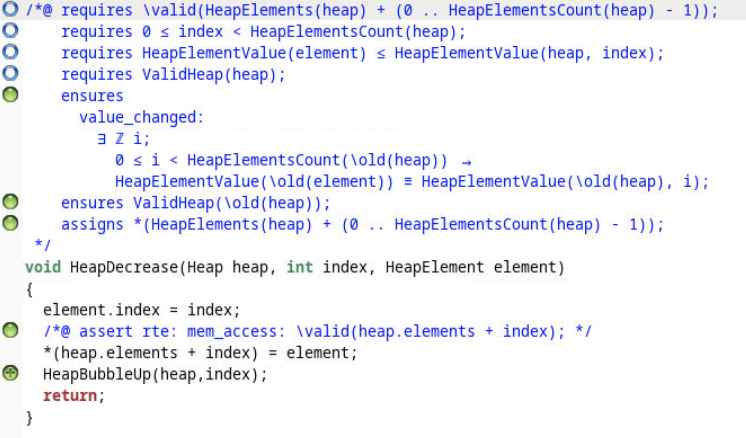
\includegraphics[width=10cm]{images/frama-c-HeapDecrease}
	\caption{Úspešné dokončení důkazu snížení hodnoty prvku haldy v prostředí Frama-C}
	\label{img:F-C-HeapDecrease}
\end{figure}


\subsection{Zvýšení hodnoty prvku}
\label{subsec:HeapIncrease}

Zvýšení hodnoty prvku haldy je operace nad haldou, která dokáže v čase $\mathcal{O}(1)$ zvýšit hodnotu vrcholu na daném indexu a následně v čase $\mathcal{O}(\log(n))$ opravit haldové uspořádání. Celková časová asymptotická složitost je tedy $\mathcal{O}(\log(n))$.

\begin{listing}[H]
	\caption{Kód a ACSL anotace zvýšení hodnoty prvku v hladě}
	\label{code:HeapIncrease}
	\begin{minted}{c}
/*@
  requires \valid(HeapElements(heap) + (0 .. HeapElementsCount(heap) - 1));
  requires 0 <= index < HeapElementsCount(heap);
  requires HeapElementValue(heap, index) <= HeapElementValue(element);
  requires ValidHeap(heap);

  assigns HeapElements(heap)[0 .. HeapElementsCount(heap) - 1];

  ensures value_changed:
    \exists integer i;
      0 <= i < HeapElementsCount(heap) ==>
        HeapElementValue(element) == HeapElementValue(heap, i);
  ensures ValidHeap(heap);
*/
void HeapIncrease(Heap heap, int index, HeapElement element) {
  element.index = index;
  heap.elements[index] = element;

  HeapBubbleDown(heap, index);
}
	\end{minted}
\end{listing}

Výpis kódu \ref{code:HeapIncrease} zobrazuje funkci pro zvýšení hodnoty prvku v haldě a~její kontrakt. Jedna ze vstupních podmínek této funkce ověřuje, že hodnota prvku, která nahrazuje původní hodnotu prvku je doopravdy vyšší nebo stejná. Pokud by tato podmínka neplatila, volání algoritmu probublání dolů by neopravilo haldové uspořádání a nebylo by možné dokončit důkaz korektnosti algoritmu. Obrázek \ref{img:F-C-HeapIncrease} zobrazuje úspěšně dokončený důkaz korektnosti algoritmu zvýšení hodnoty prvku v haldě.

\begin{figure}[H]
	\centering
	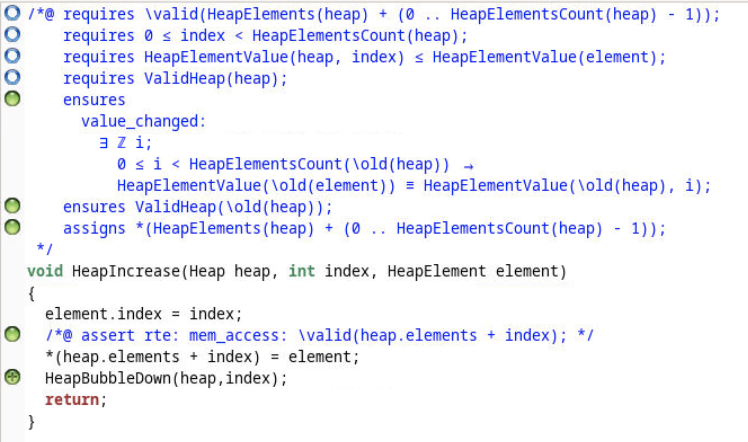
\includegraphics[width=10cm]{images/frama-c-HeapIncrease}
	\caption{Úspešné dokončení důkazu zvýšení hodnoty prvku haldy v prostředí Frama-C}
	\label{img:F-C-HeapIncrease}
\end{figure}


\section{Konstrukce haldy}
\label{subsec:HeapBuild}

Algoritmus konstrukce haldy je prvotní akce, která vytváří strukturu haldy a zajišťuje haldové uspořádání mezi prvky, ze kterých má být halda sestavena.

Implementace pomocí postupného vkládání jednotlivých prvků má časovou složitost $\mathcal{O}(n\log(n))$, jelikož musíme provést algoritmus vložení prvku, který má časovou složitost $\mathcal{O}(\log(n))$ pro každý prvek, ze kterého má být halda sestavena. \cite{IntroductionToAlgorithms2022}

Tento algoritmus lze efektivně implementovat pomocí postupného opravování haldy probubláváním rodičovských vrcholů dolů. \cite{IntroductionToAlgorithms2022} Algoritmus postupně zvětšuje podgraf spodního řezu haldou pomocí potomka až do té doby, než daný řez obsahuje všechny prvky, ze kterých měla být halda sestavena. Anotace algoritmus probublání dolů obsahují základní vstupní podmínky pro částečné opravení haldy, které tento postup splňují. Algoritmus sestavení haldy postupně nechává probublat dolů všechny rodičovské vrcholy od největšího index v poli až po kořen.

\begin{listing}[H]
	\caption{Kód a ACSL anotace zvýšení hodnoty prvku v hladě}
	\label{code:HeapBuild}
	\begin{minted}{c}
/*@
  requires 0 <= elementsCount <= elementsCapacity;
  requires \valid(elements + (0 .. elementsCount - 1));
  requires correctly_indexed:
    \forall integer i;
      0 <= i < elementsCount ==>
        HeapElementIndex(elements[i]) == i;

  assigns elements[0 .. elementsCount - 1];

  ensures count_same: HeapElementsCount(\result) == elementsCount;
  ensures capacity_same: HeapElementsCapacity(\result) == elementsCapacity;
  ensures ValidHeap(\result);
*/
Heap HeapBuild(HeapElement *elements, int elementsCount, int elementsCapacity) {
  Heap heap;
  heap.elements = elements;
  heap.elementsCount = elementsCount;
  heap.elementsCapacity = elementsCapacity;

  /*@
    loop invariant -1 <= index <= ((int)\floor(HeapElementsCount(heap) / 2)) - 1;

    loop invariant partially_valid_heap:
      \forall integer ancestor, descendant;
        index < ancestor < descendant < HeapElementsCount(heap)
        && IsParent(ancestor, descendant) ==>
          HasHeapProperty(heap, ancestor, descendant);

    loop assigns index, HeapElements(heap)[0 .. HeapElementsCount(heap) - 1];
    loop variant index;
  */
  for (int index = HeapInternalNodeCount(heap) - 1; index >= 0; index--) {
    HeapBubbleDown(heap, index);
  }

  return heap;
}
	\end{minted}
\end{listing}

Invarianty cyklu ve výpisu kód \ref{code:HeapBuild} zajišťují haldové uspořádání v spodním řezu haldou pomocí potomka s postupně snižujícím se indexem. Tento index bude po posledním kroku cyklu nastaven na hodnotu $-1$ a invariant spodního řezu haldou pomocí potomka tedy bude obsahovat celou haldu a bude zajišťovat haldové uspořádání v celé haldě.

%---------------------------------------------------------------
\chapter{Metody ladění při vývoji důkazu}
%---------------------------------------------------------------

Důkazní postupy v jazyku ACSL mohou být výrazně odlišené od matematických a formálních důkazů v knihách a publikacích. Při tvorbě nebo přepisu predikátů, konstrukci invariantů cyklů nebo při kontrole vstupních podmínek je výhodné pro vývojáře znát některé techniky, které mohou pomoci odhalit chyby v kódu nebo v důkazech. 

\section{Zúžení vstupních podmínek}

Při návrhu funkce lze definovat vstupní podmínky, které musejí být splněně, aby mohla být daná funkce spuštěna. Tato podmínka může kontrolovat například hodnoty předávaných parametrů. Pokud by funkce zaručovala platnost nějakého tvrzení při dokončení funkce, může nastat situace, že žádný z důkazních nástrojů nebude schopný danou vlastnost ověřit. Pokud se jedná o chybu v kódu nebo anotaci funkce, lze ji snadným způsobem odhalit pomocí zúžení vstupních podmínek.

Mějme definovaný induktivní predikát, který tvoří tranzitivní uzávěr haldového uspořádání v binární minimové haldě. Induktivní predikát má základní podmínky platnosti a následuje induktivně popsaná vlastnost, která může být splněna.

\begin{listing}[H]
	\caption{Chybný ACSL predikát tranzitivní vlastnosti být potomkem}
	\label{acsl:IsDescendantFail}
	\begin{minted}{c}
/*@
  inductive IsDescendant(integer descendant, integer ancestor, Heap heap) {
    case children:
      \forall integer child, Heap *heap;
        0 < child < HeapElementsCount(heap) ==>
          IsDescendant(child, Parent(child), heap);

    case descendants:
      \forall integer ancestor, element, Heap *heap;
        0 <= ancestor < element < HeapElementsCount(heap) ==>
          IsDescendant(ancestor, Parent(element), heap) ==> 
            IsDescendant(element, ancestor, heap);
  }
    \end{minted}
\end{listing}

Takto zadefinovaný predikát není správně. Pomocí prázdné funkce se vstupní podmínkou platnosti tohoto predikátu a vynuceným počtem vrcholů lze tento predikát testovat. Na obrázku \ref{img:F-C-test-IsDescendantFail} je vidět příklad použití této metody a nalezeným problém v definici predikátu. ACSL správně dokázalo predikát pro vrcholy a jejich přímé potomky, ale již nebylo možné dokázat platnosti predikátu přes více potomků. Tato informace vývojáři naznačuje, že chyba nejspíše nebude v základním případu s platností predikátu u přímých potomků vrcholů, ale bude nejspíše v induktivní části predikátu.

\begin{figure}[H]
	\centering
	
\includegraphics[width=10cm]{images/frama-c-test-IsDescendantFail}
	\caption{Neúspešné dokončení kontroly platnosti predikátu  IsDescendant v prostředí Frama-C}
	\label{img:F-C-test-IsDescendantFail}
\end{figure}


\begin{listing}[H]
	\caption{Opravený ACSL predikát tranzitivní vlastnosti být potomkem}
	\label{acsl:IsDescendantSuccess}
	\begin{minted}{c}
/*@
  inductive IsDescendant(integer descendant, integer ancestor, Heap heap) {
    case children:
      \forall integer child, Heap *heap;
        0 < child < HeapElementsCount(heap) ==>
          IsDescendant(child, Parent(child), heap);

    case descendants:
      \forall integer ancestor, element, Heap *heap;
        0 <= ancestor < element < HeapElementsCount(heap) ==>
          IsDescendant(Parent(element), ancestor, heap) ==> 
            IsDescendant(element, ancestor, heap);
  }
    \end{minted}
\end{listing}

Predikát zobrazený ve výpisu kódu \ref{acsl:IsDescendantSuccess} obsahuje opravené pořadí argumentů v předpokladu implikace. Korektnosti opravy tohoto predikátu je následně ověřena v původní funkci na obrázku \ref{img:F-C-test-IsDescendantSuccess}. Tento postup napomáhá při hledání konkrétní chyby v definici predikátu nebo funkcí. Při vývoji důkazu binární minimové haldy v této práci byla tato metoda hledání chyby nejčastější.

\begin{figure}[H]
	\centering
	
\includegraphics[width=10cm]{images/frama-c-test-IsDescendantSuccess}
	\caption{Úspešné dokončení kontroly platnosti predikátu  IsDescendant v prostředí Frama-C}
	\label{img:F-C-test-IsDescendantSuccess}
\end{figure}


\section{Kontradikce}





%\section{Důkazy s referenčními datovými typy}
%
%V průběhu tvorby autor práce předával datovou strukturu mezi jednotlivými funkcemi pomocí odkazu na paměť. Princip předávání celé datové struktury pomocí odkazu umožňuje minimalizovat počet proměnných na zásobníku a všechny hodnoty ukládá v dynamické části paměti.
%
%Datová struktura reprezentující haldu se sestává z ukazatele na začátek pole, ve kterém jsou prvky haldy uložené, celočíselné hodnoty reprezentující aktuální počet uložených prvků v haldě a maximální kapacitu alokované paměti pole.
%
%Pokud je tato struktura předaná do některé obslužné funkce, která by s některými hodnotami pracovala, Frama-C a její WP plugin nemůže zajistit, že se v průběhu provádění dané funkce hodnoty nebudou měnit. Jelikož k hodnotám uloženým v haldě přistupujeme pomocí dereference ukazatele, může se teoreticky kdykoli stát, že hodnoty v paměti, kam daný ukazatel ukazuje již nejsou aktuální. Příkladem můžou být například vícevláknové aplikace.
%
%\section{Opravení haldy probubláním nahoru}
%
%Probublání prvku nahoru potřeba provést, pokud se v některý moment objeví v haldě prvek, který nesplňuje vlastnosti haldy a hodnota v daném vrcholu je menší, než hodnota v jeho rodiči. Tento stav nastává při vkládání prvku do haldy, kde se nový prvek přidá jako poslední prvek v téměř úplném binárním stromě a provede se probublání nahoru, aby se daný prvek dostal do správného místa v haldě tak, aby byla zajištěna vlastnost haldy pro všechny vrcholy rodičů a jejich synů.
%
%\subsection{Řez haldou}
%
%Pro důkaz autor využil řez haldou, který rozděluje graf haldy dle vlastnosti haldy (hodnota v rodiči je menší nebo rovna hodnotám v jeho synech) na dvě části. Korektní halda splňuje haldovu vlastnost mezi všemi dvojicemi rodič - syn. 
%Vrchní řez haldou tento predikát omezuje pouze na syny, kteří mají index v haldě ostře menší než problematický vrchol. Pro tyto vrcholy a jejich rodiče musí platit haldová vlastnost.
%Spodní řez haldou omezuje původní predikát na vrcholy, které mají index v haldě ostře větší než problematický index a pro ně také musí platit haldová vlastnost.
%Pro algoritmus probublání nahoru musí být zajištěno, že pouze problematický vrchol jakožto syn může porušovat haldoovu podmínku se svým rodičem.
%Princip důkazu spočívá v postupném posouvání vrchního a horního řezu do té doby, než horní řez není aplikován na žádný vrchol a spodní řez je aplikován na celou haldu. Tento moment nastává při pokusu o probublání kořene haldy. Jelikož žádný syn nemůže mít menší vrchol než kořen, predikát horního řezu je triviálně splněn. Dolní řež je poté speciálním případem původního predikátu korektní haldy. Tento princip je také zefektivněn v případě, že najdeme správné místo, kde by měl problematický vrchol zůstat, haldová vlastnost určitě platí pro vrcholy v horním i spodním řezu a nově i pro správně probublaný vrchol, což zaručuje plně splněný původní predikát korektní haldy.
%
%\section{Důkaz korektnosti algoritmu opravení haldy probubláním dolů}
%
%Podobně jako v případě probublání problémového prvku nahoru je u algoritmu probublání prvku haldy dolů využit řez haldou. Oproti řezu, který byl využit pro probublání nahoru tento řez mluví o rodičích. Protože v případě problémového prvku je možné, že pro oba jeho syny bude potrebušena haldová vlastnost. Kdežto pří probublání nahoru bylo přímo jasné mezi kterou dvojicí rodič syn je vlastnost porušená.

%---------------------------------------------------------------
\chapter{Hledání nejkratší cesty}
%---------------------------------------------------------------

\section{Dijkstrův algoritmus}

Dijkstrův algoritmu je grafový algoritmus pomocí kterého lze nalézt nejkratší cestu mezi dvěma vrcholy ohodnoceného orientovaného grafu. Algoritmus předpokládá nezáporné ohodnocení hran. Algoritmus hledá nejkratší cesty z vrcholu $s$ do všech vrcholů grafu. Algoritmus poté vypisuje pouze hrany z cílového vrcholu. Použitím binární minimové haldy je asymptotická časová složitost tohoto algoritmu $\mathcal{O}(|E|\log(|V|))$.

%---------------------------------------------------------------
\chapter{Vývojové prostředí}
\label{chapter:development-environment}
%---------------------------------------------------------------

\section{Docker}

Docker a kotejnerové technologie umožňují spouštět kontejnery na společném jádře operačního systému. Liší se tímto od tradičních virtuálních strojů, které virtualizují jádro daného operačního systémů. Spuštěný kontejner se pomocí ... \cite{LinuxBible2020}

\subsection{Reverzní proxy}

\subsection{Editor kódu}

\subsection{Verifikační prostředí}

%---------------------------------------------------------------
\chapter*{Závěr}
\addcontentsline{toc}{chapter}{Závěr}
\markboth{Závěr}{Závěr}
%---------------------------------------------------------------

Tato práce se zaměřila na problematiku formálního důkazu implementace datové struktury binární minimové haldy. Podařilo se implementovat knihovnu v jazyce C s ACSL anotacemi, které dokazují korektnost jednotlivých knihovních funkcí. Použitím této knihovny lze psát nové programy, které bude možné kompletně formálně ověřit, jelikož používají formálně ověřenou knihovnu.

Formálně ověřená implementace binární minimové haldy byla použita v Dijkstrově algoritmu pro hledání nejkratší cesty v grafu. Rozšířením této práce by mohl být důkaz korektnosti tohoto algoritmu. Binární halda byla navržena pro ukládání celočíselných hodnot jednotlivých prvků, další modifikace knihovny by mohla obsahovat rozšíření pro možnost uložení desetinných čísel.

Součástí práce také vzniklo univerzální vývojové prostředí s možností editace kódu a spouštění formálního ověření bez nutnosti instalace jednotlivých programů přímo do operačního systému. Toto vývojové prostředí lze spustit na vzdáleném počítači (serveru) a následně editaci kódu a spouštění verifikace programů provádět pomocí webového prohlížeče vzdáleně.